        %%******************************************%%
        %%                                          %%
        %%        Modello di tesi di laurea         %%
        %%            di Andrea Giraldin            %%
        %%                                          %%
        %%             2 novembre 2012              %%
        %%                                          %%
        %%******************************************%%




% PDF/A filecontents
\RequirePackage{filecontents}
\begin{filecontents*}{\jobname.xmpdata}
  \Title{Document’s title}
  \Author{Author’s name}
  \Language{it-IT}
  \Subject{The abstract, or short description.}
  \Keywords{keyword1\sep keyword2\sep keyword3}
\end{filecontents*}

\documentclass[10pt,                    % corpo del font principale
               a4paper,                 % carta A4
               twoside,                 % impagina per fronte-retro
               openright,               % inizio capitoli a destra
               english,                 
               italian,                 
               ]{book}    

%**************************************************************
% Importazione package
%************************************************************** 

\PassOptionsToPackage{dvipsnames}{xcolor} % colori PDF/A

\usepackage{colorprofiles}

\usepackage[a-2b,mathxmp]{pdfx}[2018/12/22]
                                        % configurazione PDF/A
                                        % validare in https://www.pdf-online.com/osa/validate.aspx

%\usepackage{amsmath,amssymb,amsthm}    % matematica

\usepackage[T1]{fontenc}                % codifica dei font:
                                        % NOTA BENE! richiede una distribuzione *completa* di LaTeX

\usepackage[utf8]{inputenc}             % codifica di input; anche [latin1] va bene
                                        % NOTA BENE! va accordata con le preferenze dell'editor

\usepackage[english, italian]{babel}    % per scrivere in italiano e in inglese;
                                        % l'ultima lingua (l'italiano) risulta predefinita

\usepackage{bookmark}                   % segnalibri

\usepackage{caption}                    % didascalie

\usepackage{chngpage,calc}              % centra il frontespizio

\usepackage{csquotes}                   % gestisce automaticamente i caratteri (")

\usepackage{emptypage}                  % pagine vuote senza testatina e piede di pagina

\usepackage{epigraph}			% per epigrafi

\usepackage{eurosym}                    % simbolo dell'euro

%\usepackage{indentfirst}               % rientra il primo paragrafo di ogni sezione

\usepackage{graphicx}                   % immagini

\usepackage{hyperref}                   % collegamenti ipertestuali

\usepackage[binding=5mm]{layaureo}      % margini ottimizzati per l'A4; rilegatura di 5 mm

\usepackage{listings}                   % codici

\usepackage{microtype}                  % microtipografia

\usepackage{mparhack,fixltx2e,relsize}  % finezze tipografiche

\usepackage{nameref}                    % visualizza nome dei riferimenti                                      
\usepackage[font=small]{quoting}        % citazioni

\usepackage{subfig}                     % sottofigure, sottotabelle

\usepackage[italian]{varioref}          % riferimenti completi della pagina

\usepackage{booktabs}                   % tabelle                                       
\usepackage{tabularx}                   % tabelle di larghezza prefissata                                    
\usepackage{longtable}                  % tabelle su più pagine                                        
\usepackage{ltxtable}                   % tabelle su più pagine e adattabili in larghezza

\usepackage[toc, acronym]{glossaries}   % glossario
                                        % per includerlo nel documento bisogna:
                                        % 1. compilare una prima volta tesi.tex;
                                        % 2. eseguire: makeindex -s tesi.ist -t tesi.glg -o tesi.gls tesi.glo
                                        % 3. eseguire: makeindex -s tesi.ist -t tesi.alg -o tesi.acr tesi.acn
                                        % 4. compilare due volte tesi.tex.

\usepackage[backend=biber,style=numeric,hyperref,backref, maxnames=10]{biblatex}
                                        % eccellente pacchetto per la bibliografia; 
                                        % produce uno stile di citazione autore-anno; 
                                        % lo stile "numeric-comp" produce riferimenti numerici
                                        % per includerlo nel documento bisogna:
                                        % 1. compilare una prima volta tesi.tex;
                                        % 2. eseguire: biber tesi
                                        % 3. compilare ancora tesi.tex.

\usepackage{float}						% per l'opzione nelle immagini che permette
										% di posizionarle nel testo 

\usepackage{enumitem}                   % per cambiare i bullet delle liste

\setlist[itemize]{label=\textbullet}    % imposto il default per i bullet delle liste
\setlist[itemize,2]{label={--}}			% default list innestata con bullaet a -

\raggedbottom							% per evitare che il testo tenti semple di
										% occupare tutta la pagina



%**************************************************************
% file contenente le impostazioni della tesi
%**************************************************************

%**************************************************************
% Frontespizio
%**************************************************************

% Autore
\newcommand{\myName}{Riccardo Montagnin}                                    
\newcommand{\myTitle}{Titolo della tesi}

% Tipo di tesi                   
\newcommand{\myDegree}{Tesi di laurea}

% Università             
\newcommand{\myUni}{Università degli Studi di Padova}

% Facoltà       
\newcommand{\myFaculty}{Corso di Laurea in Informatica}

% Dipartimento
\newcommand{\myDepartment}{Dipartimento di Matematica "Tullio Levi-Civita"}

% Titolo del relatore
\newcommand{\profTitle}{Prof.}

% Relatore
\newcommand{\myProf}{Tullio Vardanega}

% Luogo
\newcommand{\myLocation}{Padova}

% Anno accademico
\newcommand{\myAA}{2016-2017}

% Data discussione
\newcommand{\myTime}{Luglio 2017}


%**************************************************************
% Impostazioni di impaginazione
% see: http://wwwcdf.pd.infn.it/AppuntiLinux/a2547.htm
%**************************************************************

\setlength{\parindent}{14pt}   % larghezza rientro della prima riga
\setlength{\parskip}{0pt}   % distanza tra i paragrafi


%**************************************************************
% Impostazioni di biblatex
%**************************************************************
\bibliography{bibliografia} % database di biblatex 

\defbibheading{bibliography} {
    \cleardoublepage
    \phantomsection 
    \addcontentsline{toc}{chapter}{\bibname}
    \chapter*{\bibname\markboth{\bibname}{\bibname}}
}

\setlength\bibitemsep{1.5\itemsep} % spazio tra entry

\DeclareBibliographyCategory{opere}
\DeclareBibliographyCategory{web}

\addtocategory{opere}{womak:lean-thinking}
\addtocategory{web}{site:agile-manifesto}

\defbibheading{opere}{\section*{Riferimenti bibliografici}}
\defbibheading{web}{\section*{Siti Web consultati}}


%**************************************************************
% Impostazioni di caption
%**************************************************************
\captionsetup{
    tableposition=top,
    figureposition=bottom,
    font=small,
    format=hang,
    labelfont=bf
}

%**************************************************************
% Impostazioni di glossaries
%**************************************************************
\makeglossaries

%**************************************************************
% Acronimi
%**************************************************************
\newacronym[description={\glslink{apig}{Application Program Interface}}]
    {api}{API}{Application Program Interface}

\newacronym[description={\glslink{umlg}{Unified Modeling Language}}]
    {uml}{UML}{Unified Modeling Language}

%**************************************************************
% Glossario
%**************************************************************
\newglossaryentry{apig}
{
    name=\glslink{api}{API},
    text=Application Program Interface,
    sort=api,
    description={in informatica con il termine \emph{Application Programming Interface API} (ing. interfaccia di programmazione di un'applicazione) si indica ogni insieme di procedure disponibili al programmatore, di solito raggruppate a formare un set di strumenti specifici per l'espletamento di un determinato compito all'interno di un certo programma. La finalità è ottenere un'astrazione, di solito tra l'hardware e il programmatore o tra software a basso e quello ad alto livello semplificando così il lavoro di programmazione}
}

\newglossaryentry{umlg}
{
    name=\glslink{uml}{UML},
    text=UML,
    sort=uml,
    description={in ingegneria del software \emph{UML, Unified Modeling Language} (ing. linguaggio di modellazione unificato) è un linguaggio di modellazione e specifica basato sul paradigma object-oriented. L'\emph{UML} svolge un'importantissima funzione di ``lingua franca'' nella comunità della progettazione e programmazione a oggetti. Gran parte della letteratura di settore usa tale linguaggio per descrivere soluzioni analitiche e progettuali in modo sintetico e comprensibile a un vasto pubblico}
}
 % database di termini


%**************************************************************
% Impostazioni di graphicx
%**************************************************************
\graphicspath{{immagini/}} % cartella dove sono riposte le immagini


%**************************************************************
% Impostazioni di hyperref
%**************************************************************
\hypersetup{
    %hyperfootnotes=false,
    %pdfpagelabels,
    %draft,	% = elimina tutti i link (utile per stampe in bianco e nero)
    colorlinks=true,
    linktocpage=true,
    pdfstartpage=1,
    pdfstartview=,
    % decommenta la riga seguente per avere link in nero (per esempio per la stampa in bianco e nero)
    %colorlinks=false, linktocpage=false, pdfborder={0 0 0}, pdfstartpage=1, pdfstartview=FitV,
    breaklinks=true,
    pdfpagemode=UseNone,
    pageanchor=true,
    pdfpagemode=UseOutlines,
    plainpages=false,
    bookmarksnumbered,
    bookmarksopen=true,
    bookmarksopenlevel=1,
    hypertexnames=true,
    pdfhighlight=/O,
    %nesting=true,
    %frenchlinks,
    urlcolor=webbrown,
    linkcolor=RoyalBlue,
    citecolor=webgreen,
    %pagecolor=RoyalBlue,
    %urlcolor=Black, linkcolor=Black, citecolor=Black, %pagecolor=Black,
    pdftitle={\myTitle},
    pdfauthor={\textcopyright\ \myName, \myUni, \myFaculty},
    pdfsubject={},
    pdfkeywords={},
    pdfcreator={pdfLaTeX},
    pdfproducer={LaTeX}
}

%**************************************************************
% Impostazioni di itemize
%**************************************************************
\renewcommand{\labelitemi}{$\ast$}

%\renewcommand{\labelitemi}{$\bullet$}
%\renewcommand{\labelitemii}{$\cdot$}
%\renewcommand{\labelitemiii}{$\diamond$}
%\renewcommand{\labelitemiv}{$\ast$}


%**************************************************************
% Impostazioni di listings
%**************************************************************
\lstset{
    language=[LaTeX]Tex,%C++,
    keywordstyle=\color{RoyalBlue}, %\bfseries,
    basicstyle=\small\ttfamily,
    %identifierstyle=\color{NavyBlue},
    commentstyle=\color{Green}\ttfamily,
    stringstyle=\rmfamily,
    numbers=none, %left,%
    numberstyle=\scriptsize, %\tiny
    stepnumber=5,
    numbersep=8pt,
    showstringspaces=false,
    breaklines=true,
    frameround=ftff,
    frame=single
} 


%**************************************************************
% Impostazioni di xcolor
%**************************************************************
\definecolor{webgreen}{rgb}{0,.5,0}
\definecolor{webbrown}{rgb}{.6,0,0}


%**************************************************************
% Altro
%**************************************************************

\newcommand{\omissis}{[\dots\negthinspace]} % produce [...]

% eccezioni all'algoritmo di sillabazione
\hyphenation
{
    ma-cro-istru-zio-ne
    gi-ral-din
}

\newcommand{\sectionname}{sezione}
\addto\captionsitalian{\renewcommand{\figurename}{Figura}
                       \renewcommand{\tablename}{Tabella}}

\newcommand{\glsfirstoccur}{\ap{{[g]}}}

\newcommand{\intro}[1]{\emph{\textsf{#1}}}

%**************************************************************
% Environment per ``rischi''
%**************************************************************
\newcounter{riskcounter}                % define a counter
\setcounter{riskcounter}{0}             % set the counter to some initial value

%%%% Parameters
% #1: Title
\newenvironment{risk}[1]{
    \refstepcounter{riskcounter}        % increment counter
    \par \noindent                      % start new paragraph
    \textbf{\arabic{riskcounter}. #1}   % display the title before the 
                                        % content of the environment is displayed 
}{
    \par\medskip
}

\newcommand{\riskname}{Rischio}

\newcommand{\riskdescription}[1]{\textbf{\\Descrizione:} #1.}

\newcommand{\risksolution}[1]{\textbf{\\Soluzione:} #1.}

%**************************************************************
% Environment per ``use case''
%**************************************************************
\newcounter{usecasecounter}             % define a counter
\setcounter{usecasecounter}{0}          % set the counter to some initial value

%%%% Parameters
% #1: ID
% #2: Nome
\newenvironment{usecase}[2]{
    \renewcommand{\theusecasecounter}{\usecasename #1}  % this is where the display of 
                                                        % the counter is overwritten/modified
    \refstepcounter{usecasecounter}             % increment counter
    \vspace{10pt}
    \par \noindent                              % start new paragraph
    {\large \textbf{\usecasename #1: #2}}       % display the title before the 
                                                % content of the environment is displayed 
    \medskip
}{
    \medskip
}

\newcommand{\usecasename}{UC}

\newcommand{\usecaseactors}[1]{\textbf{\\Attori Principali:} #1. \vspace{4pt}}
\newcommand{\usecasepre}[1]{\textbf{\\Precondizioni:} #1. \vspace{4pt}}
\newcommand{\usecasedesc}[1]{\textbf{\\Descrizione:} #1. \vspace{4pt}}
\newcommand{\usecasepost}[1]{\textbf{\\Postcondizioni:} #1. \vspace{4pt}}
\newcommand{\usecasealt}[1]{\textbf{\\Scenario Alternativo:} #1. \vspace{4pt}}

%**************************************************************
% Environment per ``namespace description''
%**************************************************************

\newenvironment{namespacedesc}{
    \vspace{10pt}
    \par \noindent                              % start new paragraph
    \begin{description} 
}{
    \end{description}
    \medskip
}

\newcommand{\classdesc}[2]{\item[\textbf{#1:}] #2}
                     % file con le impostazioni personali

\begin{document}
%**************************************************************
% Materiale iniziale
%**************************************************************
\frontmatter
% !TEX encoding = UTF-8
% !TEX TS-program = pdflatex
% !TEX root = ../tesi.tex

%**************************************************************
% Frontespizio 
%**************************************************************
\begin{titlepage}

\begin{center}

\begin{LARGE}
\textbf{\myUni}\\
\end{LARGE}

\vspace{10pt}

\begin{Large}
\textsc{\myDepartment}\\
\end{Large}

\vspace{10pt}

\begin{large}
\textsc{\myFaculty}\\
\end{large}

\vspace{30pt}
\begin{figure}[htbp]
\begin{center}

\includegraphics[height=6cm]{logo-unipd}
\end{center}
\end{figure}
\vspace{30pt} 

\begin{LARGE}
\begin{center}
\textbf{\myTitle}\\
\end{center}
\end{LARGE}

\vspace{10pt} 

\begin{large}
\textsl{\myDegree}\\
\end{large}

\vspace{40pt} 

\begin{large}
\begin{flushleft}
\textit{Relatore}\\ 
\vspace{5pt} 
\profTitle \myProf
\end{flushleft}

\vspace{0pt} 

\begin{flushright}
\textit{Laureando}\\ 
\vspace{5pt} 
\myName
\end{flushright}
\end{large}

\vspace{20pt}

\line(1, 0){338} \\
\begin{normalsize}
\textsc{Anno Accademico \myAA}
\end{normalsize}

\end{center}
\end{titlepage} 
% !TEX encoding = UTF-8
% !TEX TS-program = pdflatex
% !TEX root = ../tesi.tex

%**************************************************************
% Colophon
%**************************************************************
\clearpage
\phantomsection
\thispagestyle{empty}

\hfill

\vfill

\noindent\myName: \textit{\myTitle,}
\myDegree,
\textcopyright\ \myTime.
% !TEX encoding = UTF-8
% !TEX TS-program = pdflatex
% !TEX root = ../tesi.tex

%**************************************************************
% Dedica
%**************************************************************
\cleardoublepage
\phantomsection
\thispagestyle{empty}
\pdfbookmark{Dedica}{Dedica}

\vspace*{3cm}

\begin{center}
Lorem ipsum dolor sit amet, consectetuer adipiscing elit. \\ \medskip
--- Oscar Wilde    
\end{center}

\medskip

\begin{center}
Dedicato a ...
\end{center}

% !TEX encoding = UTF-8
% !TEX TS-program = pdflatex
% !TEX root = ../tesi.tex

%**************************************************************
% Sommario
%**************************************************************
\cleardoublepage
\phantomsection
\pdfbookmark{Sommario}{Sommario}
\begingroup
\let\clearpage\relax
\let\cleardoublepage\relax
\let\cleardoublepage\relax

\chapter*{Sommario}

Il presente documento descrive il lavoro svolto durante il periodo di stage, della durata di circa trecento ore, dal laureando Pinco Pallino presso l'azienda Azienda S.p.A.
Gli obbiettivi da raggiungere erano molteplici.\\
In primo luogo era richiesto lo sviluppo di ...
In secondo luogo era richiesta l'implementazione di un ... 
Tale framework permette di registrare gli eventi di un controllore programmabile, quali segnali applicati 
Terzo ed ultimo obbiettivo era l'integrazione ...

%\vfill
%
%\selectlanguage{english}
%\pdfbookmark{Abstract}{Abstract}
%\chapter*{Abstract}
%
%\selectlanguage{italian}

\endgroup			

\vfill


% !TEX encoding = UTF-8
% !TEX TS-program = pdflatex
% !TEX root = ../tesi.tex

%**************************************************************
% Ringraziamenti
%**************************************************************
\cleardoublepage
\phantomsection
\pdfbookmark{Ringraziamenti}{ringraziamenti}

\begin{flushright}{
	\slshape    
	``Life is really simple, but we insist on making it complicated''} \\ 
	\medskip
    --- Confucius
\end{flushright}


\bigskip

\begingroup
\let\clearpage\relax
\let\cleardoublepage\relax
\let\cleardoublepage\relax

\chapter*{Ringraziamenti}

\noindent \textit{Innanzitutto, vorrei esprimere la mia gratitudine al Prof. NomeDelProfessore, relatore della mia tesi, per l'aiuto e il sostegno fornitomi durante la stesura del lavoro.}\\

\noindent \textit{Desidero ringraziare con affetto i miei genitori per il sostegno, il grande aiuto e per essermi stati vicini in ogni momento durante gli anni di studio.}\\

\noindent \textit{Ho desiderio di ringraziare poi i miei amici per tutti i bellissimi anni passati insieme e le mille avventure vissute.}\\
\bigskip

\noindent\textit{\myLocation, \myTime}
\hfill \myName

\endgroup


% !TEX encoding = UTF-8
% !TEX TS-program = pdflatex
% !TEX root = ../tesi.tex

%**************************************************************
% Indici
%**************************************************************
\cleardoublepage
\pdfbookmark{\contentsname}{tableofcontents}
\setcounter{tocdepth}{2}
\tableofcontents
%\markboth{\contentsname}{\contentsname} 
\clearpage

\begingroup 
    \let\clearpage\relax
    \let\cleardoublepage\relax
    \let\cleardoublepage\relax
    %*******************************************************
    % Elenco delle figure
    %*******************************************************    
    \phantomsection
    \pdfbookmark{\listfigurename}{lof}
    \listoffigures

    \vspace*{8ex}

    %*******************************************************
    % Elenco delle tabelle
    %*******************************************************
    \phantomsection
    \pdfbookmark{\listtablename}{lot}
    \listoftables
        
    \vspace*{8ex}
\endgroup

\cleardoublepage

\cleardoublepage

%**************************************************************
% Materiale principale
%**************************************************************
\mainmatter
% !TEX encoding = UTF-8
% !TEX TS-program = pdflatex
% !TEX root = ../tesi.tex

%**************************************************************
\chapter{Introduzione}
\label{cap:introduzione}
%**************************************************************

%Introduzione al contesto applicativo.\\
%
%\noindent Esempio di utilizzo di un termine nel glossario \\
%\gls{api}. \\
%
%\noindent Esempio di citazione in linea \\
%\cite{site:agile-manifesto}. \\
%
%\noindent Esempio di citazione nel pie' di pagina \\
%citazione\footcite{womak:lean-thinking} \\

%**************************************************************

\section{Concetti chiave}
\subsection{Processi di business e process mining}
"Il \textbf{processo aziendale} (o business process) è un insieme di attività interrelate, svolte all'interno dell'azienda nell'ambito della gestione operativa delle sue funzioni aziendali, che creano valore trasformando delle risorse (input del processo) in un prodotto finale (output del processo) a valore aggiunto, destinato ad un soggetto interno o esterno all'azienda (cliente)" \cite{site:wiki-business-process}.
\\ 
Un processo è quindi caratterizzato da una sequenza di passi (attività) con lo scopo di raggiungere un obiettivo. \'E importante notare come le varie sequenze sono spesso standardizzate, di conseguenza di avranno, per la maggior parte, esecuzioni simili.
\\ 
A loro volta i processi di business sono la fonte di informazione per il process mining. 
\\
"Il \textbf{process mining} è una tecnica di process management, che permette l'analisi dei processi di business basati sui log degli eventi." \cite{site:wiki-process-mining}
\\
Il process mining quindi offre varie tecniche per estrarre informazioni utili dai log degli eventi. 
\subsubsection{Log degli eventi}
In generale un sistema informativo (che può essere un database o un ERP) genera dati realtivi agli eventi avvenuti in forma di log, tipicamente per registrare e tracciare i cambiamenti avvenuti allo stato del sistema.
Spesso questi dati sono organizzati in forma tabulare e prendono la forma di un log di eventi.
Un log di eventi (o \textit{event log}) quindi, è una collezione di dati relativi ad eventi registrata e tracciata da un sistema informativo e conservata in file strutturati (es. CSV, XES, ecc.).
Si parla di \textbf{traccia} quando ci si riferisce ad un insieme di eventi con lo stesso case id, quindi un event log può essere visto anche come una collezione di tracce.

Rappresenta l'impronta digitale elettronica delle varie operazioni aziendali. 
Va osservato che, in generale, un log non è mai direttamente utilizzabile, può infatti contenere gap, inconsistenze e ripetizioni. Si ritiene quindi necessario delle operazioni di preparazione, che permettono di filtrare e pulire i dati.

\begin{figure}[H] 
    \centering 
    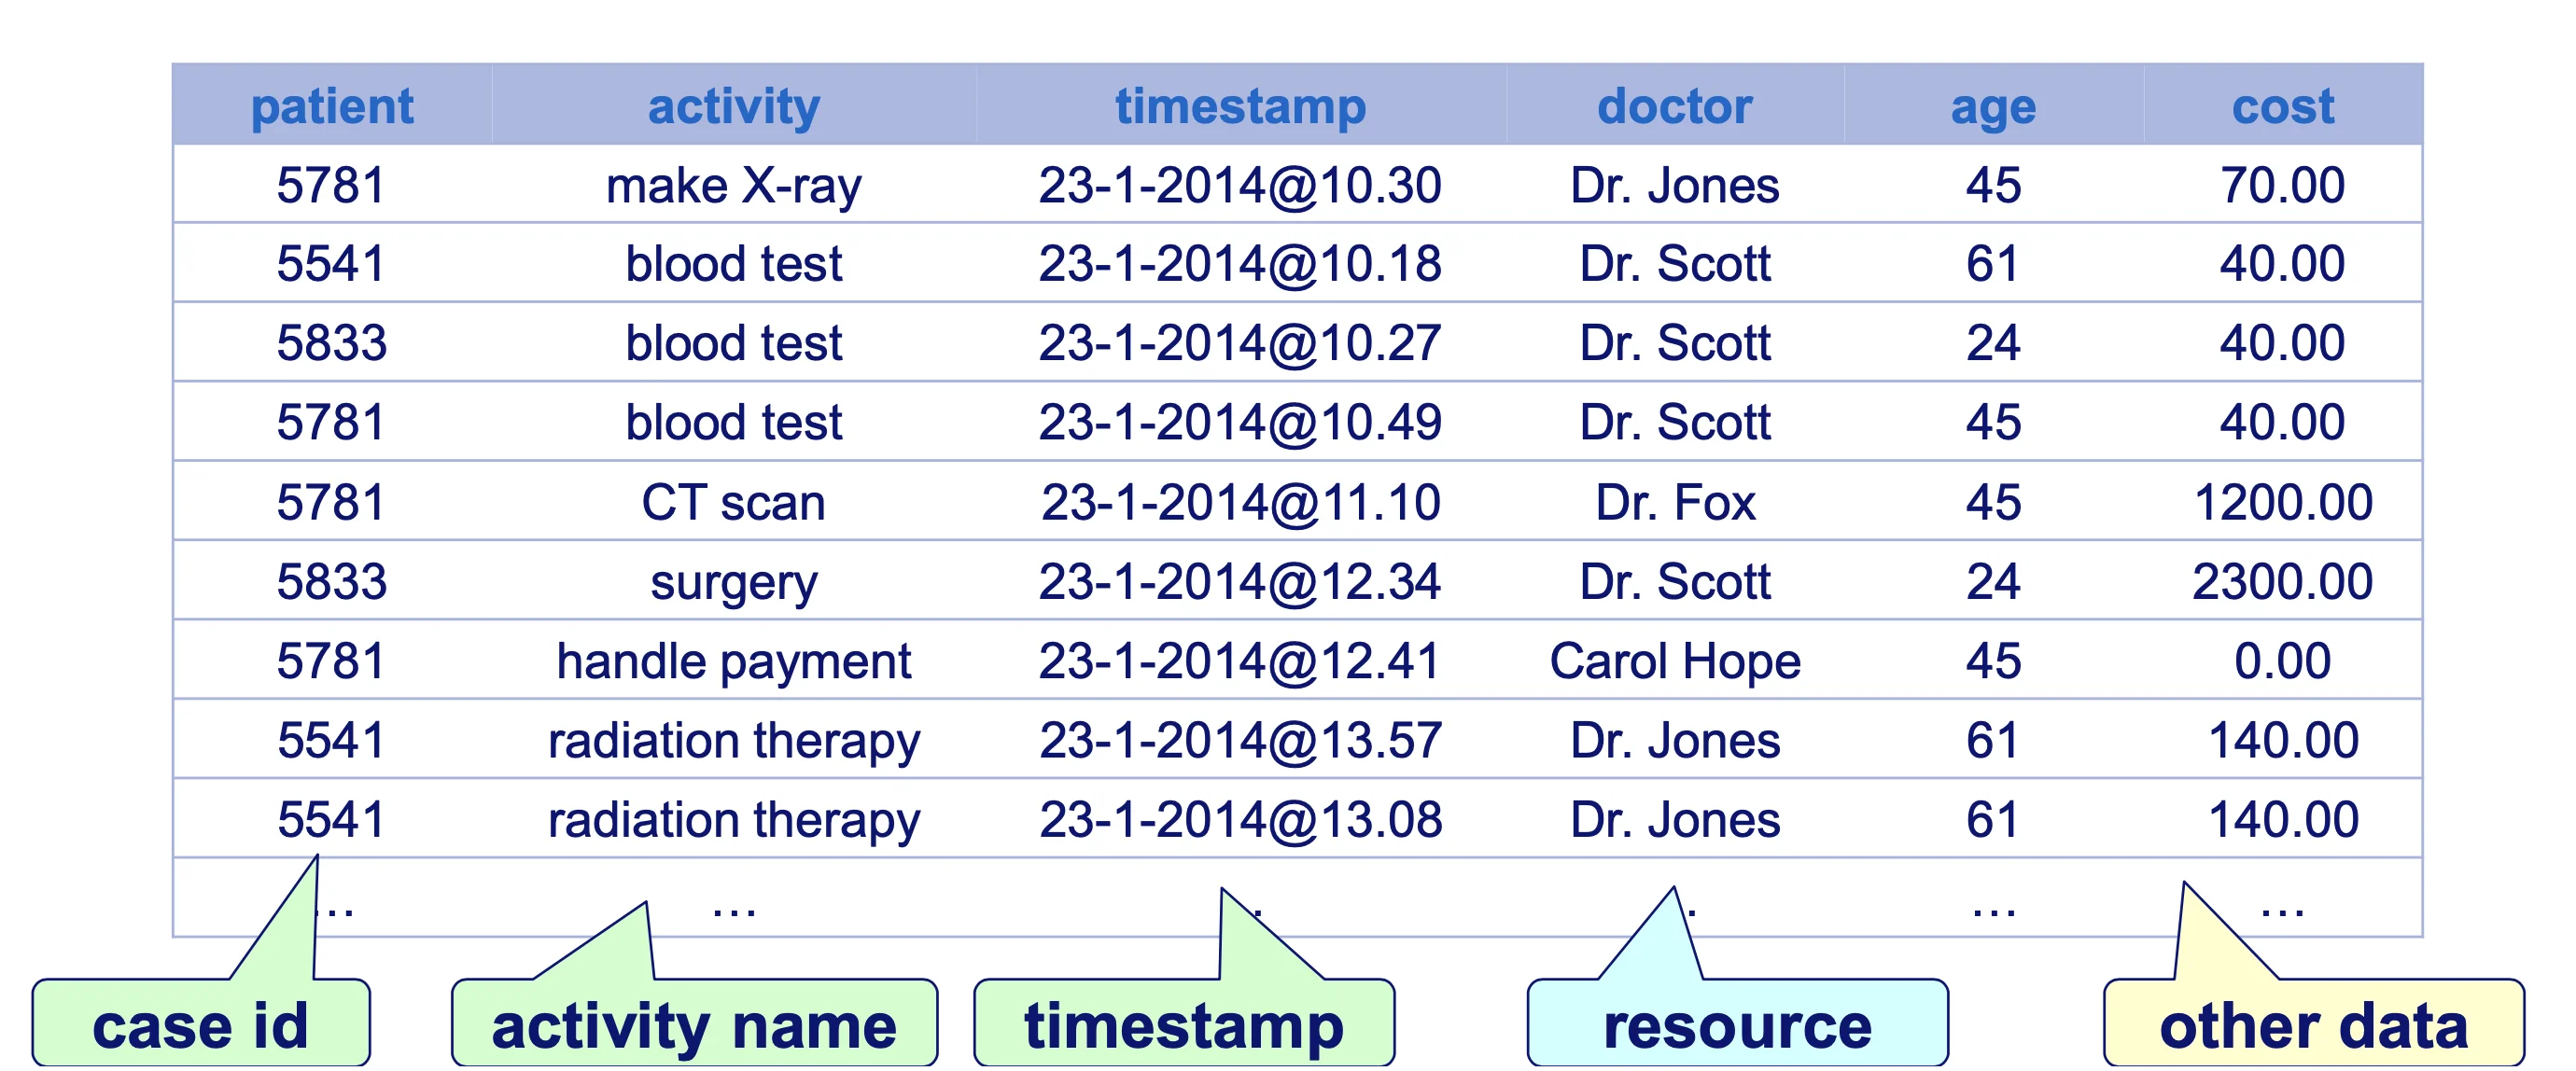
\includegraphics[width=0.9\columnwidth]{immagini/event_log_ex.png} 
    \caption{Esempio di \textit{event log} \cite{site:event-log-img}}
    \label{fig:event-log-img}
\end{figure}

Un evento (osservando la figura \ref{fig:event-log-img}) è rappresentato da una singola "riga" dell'event log, e contiene informazioni relative a:
\begin{itemize}
\item il caso trattato (identificato dal \textit{case id});
\item l'attività eseguita;
\item il riferimento temporale (\textit{timestamp}).
\end{itemize}
Importante notare come, i campi appena elencati, siano essenziali per descrivere un processo e necessari per rendere un event log utilizzabile in attività di process mining.
Ma un evento può contenere anche altre informazioni aggiuntive (es. risorse, costi, ecc.), queste non sono strettamente necessarie per modellare un processo ma sono comunque utili per effettuare analisi su prospettive diverse.

\subsubsection{Tecniche di process mining}
Le tecniche di process mining si occupano principalmente di:
\begin{itemize}
\item \textit{Process discovery}, con lo scopo di generare un \textit{process model}, ovvero una rappresentazione grafica di un processo, permettendone per la visualizzazione, la documentazione e l'estrazione di informazioni;

\item \textit{Conformance checking}, che confronta il process model con un event log per individuare le differenze e deviazioni, può anche essere utilizzato per valutare la qualità del process model generato durante l'attività di discovery, oppure individuare colli di bottiglia;

\item \textit{Enhancement}, ovvero il miglioramento del process model attraverso l'introduzione di nuove informazioni (es. misure relative alle performance).
\end{itemize}

\begin{figure}[H] 
    \centering 
    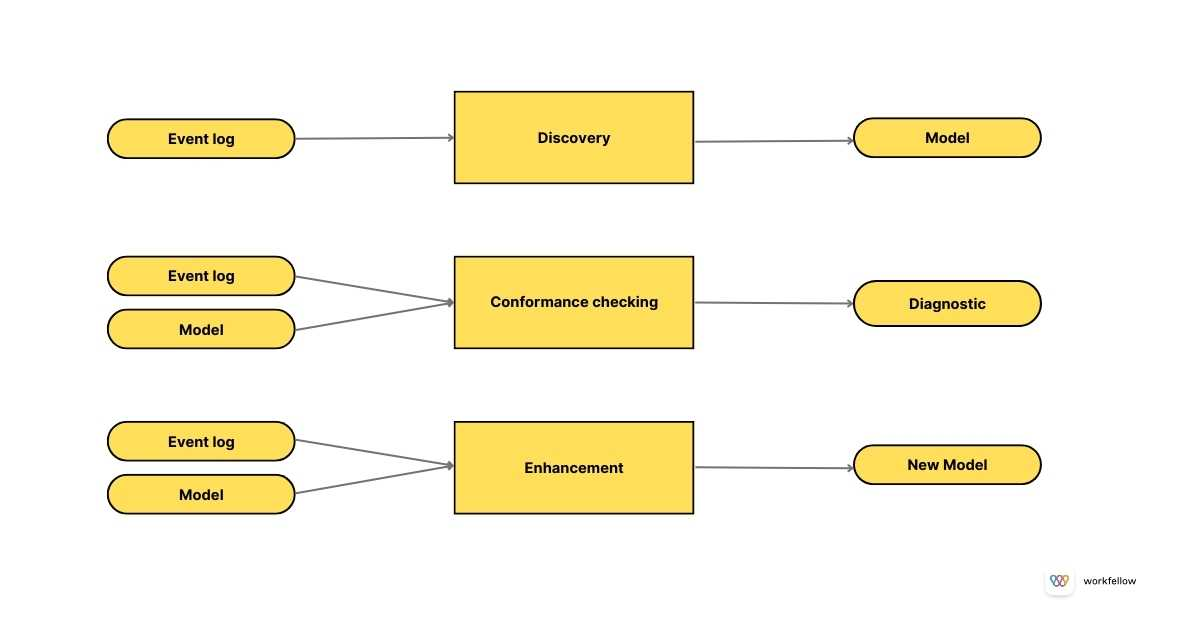
\includegraphics[width=0.9\columnwidth]{immagini/process_mining_techniques.jpg} 
    \caption{3 tipi di attività nel process mining, con relativi input e output \cite{site:process-mining-techniques-img}}
\end{figure}

Le tecniche appena descritte hanno il potenziale di generale un grande valore aggiunto. La creazione di un modello che descrive i processi rende l'individuazione di processi ripetitivi e inefficienti più semplice, permettendo di agire su di essi. Il modello a sua volta può continuamente essere affinato con informazioni aggiuntive che permettono di analizzare le performance e costruire workflow più efficienti. Lo stesso modello può poi essere comparato con event log successivi per individuare deviazioni, mostrando dove, quando e perché accadono. 
\\
Ovviamente, oltre a individuare i problemi e i punti deboli ottimizzabili, il process mining permette anche di scovarli in maniera precoce.
\\
Riassumendo, l'applicazione delle tecniche offerte dal process mining offre vantaggi come: l'ottimizzazione del workflow, la riduzione dei costi, incremento della qualità di beni o servizi offerti e la crescita della soddisfazione del cliente.


\subsection{Predictive Process Monitoring}
Il \textit{Predictive Process Monitoring} rientra tra le attività di Enhancement, ed è una branca del process mining che ha lo scopo di predire il futuro di una esecuzione in corso (e quindi ancora incompleta) di un processo \cite{pm-handbook}.
\\
Generalmente si è interessati a fare predizioni sul tempo totale di esecuzione, sulle attività successive o sui risultato finale del processo.
\\
Questo permette di ottimizzare le operazioni di business, riducendo i costi e i rischi. Inoltre rende la pianificazione in materia di allocazione delle risorse disponibili più semplice ed efficiente.
Importante è anche i benefici relativi alla soddisfazione del cliente: posso fare predizioni relative alle aspettative dei clienti o prevedere il risultato finale di un processo, offrendo tempi di attesa più certi. 
\\
Come osservato in \cite{pm-handbook}, in generale il Predictive Process Monitoring è svolto in due fasi:
\begin{itemize}
\item la fase di \textit{training}: dove viene allenato un modello predittivo (tramite tecniche di Machine Learning) su dati storici di esecuzione, dove le tracce sono complete;
\item la fase di \textit{runtime}: dove il modello predittivo creato viene interrogato con lo scopo di ottenere predizioni relative a tracce incomplete e/o in corso di esecuzione.
\end{itemize}

\subsection{Prescriptive Process Monitoring}
Va osservata la differenze tra predizione, ovvero un'affermazione che spiega ciò che, probabilmente, avverrà (o meno) in futuro e una raccomandazione, ovvero un'affermazione che spiega quale sia la miglior azione da scegliere.
Lo scopo finale del Predictive Process Monitoring è infatti, quello di offrire una predizione relativa all'ottenimento di un risultato positivo, ma non dice niente in relazione a quale sia l'azione successiva migliore da effettuare.
\\
Il Prescriptive Process Monitoring si pone questo obiettivo, supportando e offrendo raccomandazioni agli stakeholder per prevenire risultati indesiderati o per determinare quali sono le migliori attività da eseguire per ottimizzare determinati aspetti di interesse \cite{pm-handbook}.


\subsection{Sistema di raccomandazione per istanze di processi aziendali}
Un sistema di raccomandazione per istanze di processi aziendali, o PAR, è una tipologia di sistema informativo che ha lo scopo di prevedere come le istanze di processi andranno ad evolversi e raccomandare le azioni necessarie per correggere le istanze con il rischio più alto di non raggiungere il risultato desiderato, definito in termini di \gls{KPI} \cite{paper-padella}.
\\
Un sistema PAR (come descritto in \cite{paper-padella}) è composto da due sotto-sistemi: il Predictive Process Monitoring che si occupa di generare le predizioni e il Prescriptive Process Monitoring che genera le raccomandazioni relative alle azioni correttive da applicare.
\\
Sempre in \cite{paper-padella} viene fatta un'importante osservazione: le raccomandazioni, se non correttamente spiegate, spingono l'utente a diffidare di esse, aumentando il rischio che queste non vengano applicate, dato che i responsabili preferiranno prendere decisioni soggettive non fidandosi del sistema.
\\
Quindi la sola raccomandazione non basta, è importante che le ragioni che la determinano siano spiegate e rese comprensibili, così da far sentire l'utente partecipe nelle decisioni prese dal sistema e di conseguenza aumentare la fiducia in esso.
\\
Le spiegazioni del sistema proposto in \cite{paper-padella} si basano su caratteristiche relative al processo come il valore delle sue variabili, le attività effettuate e le risorse sfruttate per svolgere le attività. Il sistema utilizza i valori di Shapley (in inglese \textit{Shapley Values}) per fornire le spiegazioni, concentrandosi solamente sugli aspetti il cui impatto negativo viene maggiormente mitigato della raccomandazione.


\subsubsection{Shapley Values}
Gli Shapley Values nascono nell'ambito della teoria dei giochi, e rappresentano un approccio per suddividere equamente la ricompensa tra i giocatori che hanno collaborato in un gioco cooperativo \cite{site:wiki-shapley-values}. Servono quindi per quantificare la contribuzione che ogni giocatore ha portato al gioco stesso. In \cite{paper-padella} viene spiegato come le caratteristiche di un istanza di processo corrispondano ai giocatori, e la differenza tra la predizione fatta dal modello predittivo e la predizione media è la ricompensa. Quindi il valore di Shapley di una caratteristica di una predizione rappresenta quanto essa contribuisce a variare la predizione del modello da quella media.

\section{Struttura del resto della relazione}
%TODO

             % Introduzione
% !TEX encoding = UTF-8
% !TEX TS-program = pdflatex
% !TEX root = ../tesi.tex

%**************************************************************
\chapter{Descrizione dello stage}
\label{cap2}
\section{Scopo dello stage}
L'idea dello stage nasce dalla necessità di sviluppare una nuova interfaccia grafica front-end per un sistema di raccomandazione per le istanze di processi aziendali.
\\
Il back-end del sistema è stato precedentemente sviluppato dal dottorando Alessandro Padella, come parte del suo lavoro di tesi di dottorato (\cite{paper-padella}). 
\\
Il back-end è un PAR (vedasi \autoref{subsec:par-ref}) che implementa l'analisi prescrittiva, e ha lo scopo di raccomandare le migliori opzioni di decisione nell'ambito dei processi aziendali. Per fare questo vengono sfruttati, in particolare, i risultati dell'analisi predittiva, algoritmi di ottimizzazione e intelligenza artificiale. Le opzioni vengono individuate in termini di KPI (tempo totale di esecuzione e numero di volte in cui una specifica attività si verifica). Infine il sistema genera anche le spiegazioni (sotto forma di Shapley Values) per le raccomandazioni individuate.
\\
Lo scopo sarà quindi di sviluppare un'interfaccia grafica per il sistema, che si occupi di tutte le fasi necessarie: 
\begin{itemize}
\item caricamento dell'event log storico su cui allenare il modello;
\item selezione delle opzioni relative all'allenamento del modello desiderate dell'utente;
\item caricamento dell'event log incompleto su cui fare le predizioni;
\item visualizzazione delle predizioni, delle raccomandazioni e delle relative spiegazioni.
\end{itemize}

\section{Contenuti formativi}
Durante il progetto di stage sono state approfondite le conoscenze nei seguenti ambiti:
\begin{itemize}
\item Process mining; 
\item Progettazione e sviluppo di interfacce grafiche;
\item Framework per la data visualization;
\end{itemize}

\section{Obiettivi}
Si farà riferimento agli obiettivi secondo le seguenti notazioni:
\begin{itemize}
	\item O per i requisiti obbligatori, vincolanti in quanto obiettivo primario richiesto dal committente;
	\item D per i requisiti desiderabili, non vincolanti o strettamente necessari,
		  ma dal riconoscibile valore aggiunto;
	\item F per i requisiti facoltativi, rappresentanti valore aggiunto non strettamente 
		  necessario.
\end{itemize}
Le sigle precedentemente indicate saranno seguite da un numero sequenziale, identificativo dell'obiettivo.
\\
Lo stage prevedeva inizialmente i seguenti obiettivi:
\begin{itemize}
	\item Obbligatori
	\begin{itemize}
		\item \underline{\textit{O01}}: Produzione di un mock-up che illustra le diverse schermate che costituiscono l'interfaccia grafica;
	 \item \underline{\textit{O02}}: Produzione di diagrammi per i casi di uso considerati;
	\item \underline{\textit{O03}}: Documento di almeno quattro pagine che riassume i diversi framework analizzati con relativi pro e contro di ognuno e discute il framework scelto, motivando la scelta;
	 \item \underline{\textit{O04}}: Definizione e utilizzo delle \gls{API} di back-end, con il supporto di diagrammi di classe e diagrammi di sequenza;
\item \underline{\textit{O05}}: Sviluppo della prima versione del codice per lo sviluppo dell'interfaccia grafica e per la comunicazione con le \gls{API} di back-end;
\item \underline{\textit{O06}}: Definizione ed esecuzione dei casi di test (di unità, di interfaccia, ecc.);
\item \underline{\textit{O07}}: Sviluppo della versione finale del codice per lo sviluppo dell'interfaccia grafica e per la comunicazione con le \gls{API} di back-end;
\item \underline{\textit{O08}}: Rilascio e deployment del codice finale dopo ultima validazione.
	\end{itemize}
	
	\item Desiderabili 
	\begin{itemize}
		\item \underline{\textit{D01}}: Validazione delle \gls{API} di back-end. 
	\end{itemize}
	
	\item Facoltativi
	\begin{itemize}
		\item \underline{\textit{F01}}: Stesura documentazione.
	\end{itemize} 
\end{itemize}


\clearpage

\section{Pianificazione del lavoro}
Il periodo di svolgimento dello stage è stato dal 10 ottobre 2022 al 10 febbraio 2023, svolto in part-time, per la durata totale di 320 ore. Il part-time consisteva nello svolgere 4 ore di lavoro al giorno, per 5 giorni alla settimana, per un totale di 20 ore di lavoro settimanali.
Infine sono state considerate le 2 settimane di ferie natalizie.
\\
La pianificazione delle attività settimanali era la seguente:
  \begin{itemize}
	
        \item[] \textbf{Dalla prima alla quarta settimana (80 ore)} 
	\begin{itemize}
            	\item{Studio del problema};
	 	\item{Sviluppo di mock-up e casi d'uso};
	\end{itemize}
       

        \item[] \textbf{Dalla quinta alla settima settimana (60 ore)} 
	\begin{itemize}
            	\item{Ricerca e studio di framework grafici e visualizzazioni dati};
	 	
	\end{itemize}
        
	\item[] \textbf{Dall'ottava alla nona settimana (40 ore)}
	\begin{itemize}
            	\item {Studio e definizione di \gls{API} per il back-end};
	\end{itemize}
        
       \item[] \textbf{Dalla decima alla dodicesima settimana (60 ore)} 
	\begin{itemize}
            	\item {Sviluppo di un primo prototipo};
	\end{itemize}
        
        \item[] \textbf{Tredicesima Settimana (20 ore)} 
	\begin{itemize}
            	\item{Validazione del prototipo};
	 	
	\end{itemize}
        
        
        \item[] \textbf{Dalla quattordicesima alla quindicesima settimana (40 ore)} 
        
	\begin{itemize}
            	\item{Sviluppo del prodotto finale (che elimina le criticità osservate nei test effettuati nella tredicesima settimana)};

	\end{itemize}

         \item[] \textbf{Sedicesima Settimana (20 ore)}   
	\begin{itemize}
            	\item{Validazione e collaudo finale};
	\end{itemize} 

 \end{itemize}


\section{Variazioni alla pianificazione originale}
Durante lo svolgimento dello stage sono state applicate delle modifiche alla pianificazione e agli obiettivi da raggiungere. Tutto ciò in relazione al framework che è stato scelto per svolgere il progetto, che sarà approfondito nella \autoref{sec:analisi-framework}. Grazie ad esso l'\gls{API} per la comunicazione tra front-end e back-end si è resa non necessaria.
In particolare l'attività pianificata nell'ottava e nella nona settimana è stata sostituita con la seguente attività: sviluppo di un primo prototipo;
\\
Per quanto riguarda gli obiettivi sono stati modificati nel seguente modo:
	\begin{itemize}
    \item \underline{\textit{O04}} è stato sostituito con: Definizione architettura generale con il supporto di diagrammi di classe;
    \item \underline{\textit{O05}} e \underline{\textit{O07}} sono stati aggiornati, rimuovendo la parte relativa allo sviluppo delle \gls{API};
    \item \underline{\textit{D01}} è stato sostituito con: Implementazione funzionalità multiutente.
	\end{itemize}


\section{Organizzazione dello stage}
Una volta ogni due settimane sono stati organizzati incontri diretti con il tutor esterno, il Prof. Massimiliano de Leoni, per verificare lo stato di avanzamento del progetto, chiarire eventualmente gli obiettivi o i dubbi sorti, affinare la ricerca e aggiornare il piano di lavoro. Il tutor esterno è stato coadiuvato dal Dott. Alessandro Padella, che si è reso disponibile con frequenza anche settimanale per dare supporto nello sviluppo del progetto.



 

             % Processi
% !TEX encoding = UTF-8
% !TEX TS-program = pdflatex
% !TEX root = ../tesi.tex

%**************************************************************
\chapter{Tecnologie utilizzate}

\section{Panoramica generale}
Durante la realizzazione del progetto sono state utilizzate le seguenti tecnologie e strumenti:

\subsubsection{Git} 
Git è un sistema di controllo di versione open source per la gestione di progetto di qualsiasi dimensione in maniera rapida ed efficiente. 

\subsubsection{Github}
GitHub è un servizi di hosting basato sul cloud che permette di gestire i progetti basati sul sistema di controllo versione Git. Oltre alle funzionalità di versionamento, offre funzionalità come issue tracking e continuous integration. 


\subsubsection{Python}
Python è un linguaggio di alto livello, general-purpose, dinamicamente tipizzato e garbage-collected. Nasce intorno al 1980 da Guido van Rossum, come sostituto del linguaggio di programmazione ABC. Per lo sviluppo del progetto è stata utilizzata la versione 3.9 del linguaggio.


\subsubsection{PyCharm Community Edition}
PyCharm Community Edition è un ambiente di sviluppo integrato open-source, specializzato nello sviluppo di progetti Python. Sviluppato da JetBrains, offre syntax highlighting, auto indentazione, code completion, controllo ortografia e un debugger Python built-in.

\subsubsection{\LaTeX}
\LaTeX{} è un linguaggio dichiarativo per la stesura di documenti. \'E stato usato per la
stesura dei vari documenti richiesti per il progetto di stage.


\subsubsection{StarUML}
StarUML è un software utilizzato per modellare diagrammi \gls{UML}.
\'E stato sviluppato da MKLabs ed è disponibile per Windows, Linux and MacOS.



\section{Analisi framework proposti}
\label{sec:analisi-framework}
\subsection{Dash}

\begin{figure}[H]
    \centering
    
\includegraphics[scale=0.4]{immagini/logo_dash.png}
   \caption{Logo Dash}
\end{figure}


Dash è un microframework open source sviluppato in Python annunciato nel 2017. Viene utilizzato per la visualizzazione dati e in generale per la creazione di applicazioni web per l'analisi dati.
Dash utilizza internamente le tecnologie Flask, Plotly.js e React.js.
\\
Un'app Dash è essenzialmente un'istanza di server Flask che comunica con i client tramite HTTP con pacchetti JSON, usando React.js per il front-end e in particolare sfrutta Plotly.js per la gestione dei grafici.

\subsubsection{Vantaggi e punti di forza}
Alcuni tra i punti di forza e vantaggi individuati sono:
\begin{itemize}
\item Non richiede l'utilizzo di HTML/CSS o Javascript aggiuntivi, in quanto ogni componente in Dash codifica tutte le proprietà di uno specifico componente di React;
\\
Sono infatti presenti classi Python che codificano la maggior parte dei tag HTML (tramite \textit{dash\_html\_component}) e tutti i componenti interattivi di base offerti da React (Slider, Dropdown, Graph, ...), tramite \textit{dash\_core\_components} \cite{site:dash-core-comp};

\item Dash supporta l'aggiunta di nuovi componenti, creando un oggetto sopra a componenti preesistenti in React o definendo un proprio componente personalizzato tramite HTML/CSS e Javascript;

\item Pur facendo uso di fogli di stile di default, supporta l'aggiunta di fogli di stile CSS esterni, quindi ogni elemento è personalizzabile usando le \gls{API} offerte da Dash, oppure introducendo i propri fogli di stile, garantendo il massimo livello di personalizzazione possibile;

\item Il codice è dichiarativo e reattivo, e questo semplifica molto lo sviluppo di applicazioni (anche complesse) con numerosi componenti interattivi;

\item L'istanza di Flask alla base del server, resta totalmente accessibile, permettendo la modifica di tutte le sue proprietà configurabili. Inoltre può essere estesa (a seconda dei bisogni) con tutta una serie di plugin Flask;

\item Ottima visualizzazione degli errori per il debugging; in particolare non vengono nascosti nella console Javascript, ma evidenziati nelle grafica dell'applicazione, quando è in modalità di debug. Vengono anche isolati dalle eccezioni generate da Flask internamente, permettendo una netta distinzione tra un errore causato da Flask o da Dash;

\item Tracciamento efficace delle callback; Dash crea una visualizzazione grafica dell'albero delle callback, indicando quando sono state eseguite, per quanto hanno operato e i dati che sono stati passati.
Questo si prova molto utile, soprattutto in applicazioni medio-grandi, dove il numero di callback può diventare notevole rapidamente;

\item Dash salva lo stato dell'applicazione nel client, cioè nel browser, questo permette di avere dashboard che supportano più utenti in simultanea, permettendo di avere interazioni indipendenti con la stessa applicazione e riducendo le risorse necessarie per un nuovo utente dal lato server;

\item La presenza di più community attive e molto materiale informatico e formativo, all'infuori della documentazione;

\item Molto utilizzato e riconosciuto in ambito aziendale, tanto da offrire un'opzione premium a pagamento, Dash Enterprise.

\end{itemize}

\subsubsection{Svantaggi e punti di debolezza}
Alcuni tra i punti di debolezza individuati sono:
\begin{itemize}
\item L'aggiornamento costante di elementi grafici può diventare rapidamente oneroso vista l'architettura sopra la quale è sviluppato, dato che non avendo una cache lato server vanno comunque rifatti tutti i calcoli necessari anche se i dati non sono cambiati;

\item Dash rimane molto chiuso ad integrazioni con altre librerie grafiche, dato che per design l'unica supportata rimane Plotly.js, questo può essere limitante a seconda delle applicazioni;

\item La creazione di applicazioni multi pagina è stata resa disponibile di recente (prima non era esplicitamente supportata e c'era il bisogno di sviluppare soluzioni non standard e poco stabili), e rimane limitata. Ad esempio lo scambio di dati tra le pagine dell'applicazione deve essere sviluppato esplicitamente (visto che Dash è stateless) e può diventare complesso in poco tempo e provocare una riduzione delle performance;

\item L'interattività offerta da Dash, seppur funzionale e concisa, rimane limitata, sia per opzioni (solo callback collegate a cambi di proprietà dei componenti) che per funzionalità, per esempio non è possibile che due o più callback aggiornino lo stesso elemento. 
\\
Questo può portare a soluzioni macchinose e poco eleganti (passaggio di argomenti aggiuntivi come identificativi e definire una grande callback che accetta tutti gli input e output e con una logica complessa per ritornare la risposta corretta, mescolando comportamenti e funzionalità logicamente separate tra di loro);


\item Può richiedere conoscenze rudimentali di HTML (e CSS per un design "grafico" migliore e personalizzazione maggiore). Non sono strettamente necessarie, finché la dimensione dell'applicazione che si vuole sviluppare rimane ridotta, però con il crescere di quest'ultima possono diventarlo. A queste si aggiunge la necessità di conoscere Javascript se si vuole deviare dai comportamenti standard dei componenti;

\item In generale, anche dovuto a quanto detto nel punto sopra, lo sviluppo in Dash può diventare complesso, soprattutto appena ci si sposta su layout più complicati;

\item Difficoltà nel deployment, dato che per un'applicazione Dash il deploy avviene solo nelle piattaforme che supportano Flask, inoltre necessita un setup non triviale dell'ambiente di esecuzione, e su questi aspetti la documentazione è scarsa;

\item Dash non supporta molte funzionalità relative all'accessibilità per la maggior parte dei componenti di default offerti e per i grafici renderizzati con Plotly.js.
	
\end{itemize}

\subsection{Panel}

\begin{figure}[H]
    \centering
    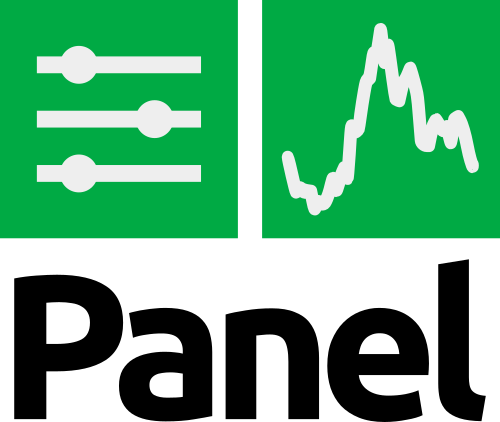
\includegraphics[scale=0.4]{immagini/logo_panel.png}
   \caption{Logo Panel}
\end{figure}


Panel è una libreria Python open source, annunciata nel maggio del 2019, che permette di creare applicazioni web interattive e dashboard personalizzate.
Panel è costruito sopra due librerie principali: 
\begin{itemize}
	\item Bokeh, un framework che implementa il pattern MVC su cui si basa Panel; offre anche alcuni componenti base, un layout manager e un server Tornado per la comunicazione tra Python e browser (usando Websocket);
	
	\item Param, un framework per definire parametri reattivi, usati per definire tutti i componenti di Panel.

\end{itemize}

\subsubsection{Vantaggi e punti di forza}
Alcuni tra i punti di forza e vantaggi individuati sono:
\begin{itemize}
\item Panel è stato pensato per essere utilizzato puramente in Python, rendendo non necessaria neanche una minima conoscenza di HTML/CSS e Javascript;

\item Panel può interfacciarsi con praticamente tutte le librerie di plotting più comuni (es. Plotly.js, matplotlib, ...);

\item Panel si interfaccia nativamente anche con molti degli strumenti connessi all'analisi dati (es. Pandas, Dusk, Datashader, ...);

\item Ottimo supporto per la creazione di applicazioni multi-pagina, tramite l'utilizzo di Pipelines, che permettono la facile definizione di un workflow, dove lo stadio precedente passa i dati allo stadio successivo;

\item Offre potenti \gls{API} per i bisogni di ogni sviluppatore \cite{site:panel-apis}:
	\begin{itemize}
		\item Interact functions: genera un'interfaccia grafica in automatico, data una funzione (la più semplice ma meno personalizzabile);
		
		\item Reactive functions: simile ad Interact functions, ma richiede che i componenti siano dichiarati in maniera esplicita e che i collegamento tra componenti e funzioni sia esplicito;
		
		\item Parameterized classes: tramite Param, permette di definire classi parametrizzate (dove vengono dichiarati i parametri e i loro intervalli), indipendenti dall'interfaccia grafica, che sarà poi generata da Panel. Questo determina molte ottimizzazioni e soprattutto una funzionalità di validazione dei parametri già pronta all'uso (tramite Param);
		
		\item Callbacks: l'interfaccia grafica viene generata dichiarando tutti i componenti necessari e ogni callback necessaria per interazione e l'aggiornamento (il metodo più "vicino" alla macchina, quindi più complesso ma più personalizzabile).
	
	\end{itemize}
	
Questo determina un elevato grado di flessibilità di sviluppo;

\item L'architettura su cui Panel è costruito salva lo stato per ogni utente e sessione sia nel server che nel client (browser) e se necessario è possibile sincronizzarli. Questo ha importanti implicazioni, permette infatti di salvare in una cache lato server le computazioni intermedie per ogni utente e rende l'applicazione molto più responsive, permettendo un'esplorazione continua di una visualizzazione con rallentamenti anche impercettibili, perché vengono ricalcolati solo i passaggi necessari; 

\item Panel renderizza l'applicazione tramite l'utilizzo di un template di default ma offre la possibilità di inserire nuovi template personalizzati e sviluppati dall'utente, permettendo il controllo sul layout di ogni singolo componente.

\end{itemize}



\subsubsection{Svantaggi e punti di debolezza}
Alcuni tra i punti di debolezza individuati sono:
\begin{itemize}
\item L'architettura sulla quale è sviluppato non scala molto bene se l'applicazione richiede di supportare una molteplicità di utenti simultanei, in quanto può velocemente saturare le risorse del server;

\item Similmente a Dash, la difficoltà di utilizzo aumenta di molto se le applicazioni e i layout diventano più complessi. In generale Panel ha una curva di apprendimento più complessa rispetto a Dash;

\item La quantità di materiale informativo e formativo disponibile (non considerando la documentazione) è considerevolmente minore rispetto a Dash. Alcuni dei motivi sono il fatto che Dash è uscito 2 anni prima di Panel, e vista la presenza di Dash Enterprise, si è venuta a una comunità più numerosa;

\item L'attività di debugging viene resa più complessa (rispetto a Dash) per la mancanza di un interfaccia chiara per la visualizzazione degli errori che sono mostrati nella console Javascript come errori o eccezioni delle librerie interne al framework. Questo rende più difficile, rispetto a Dash, la comprensione di cosa causa l'errore in caso essi siano non triviali. Di recente è stata introdotta un Debugging widget, che pur mitigando il problema resta limitata;

\item Difficoltà nel deployment, dove Panel ha comunque un numero più vasto di piattaforme sulla quale si può effettuare il deploy, resta il problema della scarsa documentazione, che manca di profondità (le varie opzioni sono discusse solo brevemente);

\item La presenza di molteplici \gls{API} di sviluppo può portare (soprattutto degli sviluppatori alle prime armi con il framework) ad effettuare delle scelte sbagliate, richiedendo in un tempo successivo un grande sforzo di refactoring.

\end{itemize}

\subsection{Scelta framework e motivazioni}
In accordo con il proponente, è stato scelto di utilizzare il framework Dash. In un primo momento si era deciso di usare Panel, ma lo sviluppo di un piccolo \gls{PoC} ha reindirizzato la scelta.
\\
In particolare le motivazioni (alcune personali) sono:
\begin{itemize}
\item Difficoltà nel debugging di Panel rispetto a Dash: come spiegato sopra, il fatto che Panel visualizzi principalmente gli errori e le eccezioni delle librerie interne, rendeva il processo di individuazione dei bug inevitabilmente lungo e tedioso. Ho invece trovato l'interfaccia offerta da Dash per la visualizzazione delle eccezioni più chiara e diretta, senza contare l'utilità delle mappa grafica dell'esecuzione delle callback generata da Dash, che invece in Panel era completamente assente;

\item Alcuni punti di debolezza di Dash sono stati mitigati, tramite le Dash Extensions \cite{site:dash-ext}. In particolare il \texttt{MultiplexerTransform}, che permette di definire più callback con lo stesso output, migliorando la definizione delle callback e permettendo la suddivisione delle funzionalità;

\item La scarsa presenza di materiare formativo e informativo per Panel e la ridotta documentazione rispetto a Dash, è stata forse la motivazione che ha avuto più impatto nella scelta del framework. Infatti la presenza di un ottimo forum \cite{site:dash-forum}, di numerose guide online e di componenti aggiuntivi non standard già sviluppati si sono rivelati di fondamentale importanza e utilità.

\end{itemize}
             % Kick-Off
% !TEX encoding = UTF-8
% !TEX TS-program = pdflatex
% !TEX root = ../tesi.tex

%**************************************************************
\chapter{Analisi dei requisiti}
\label{cap4}
%**************************************************************
 

\section{Analisi dei casi d'uso}

Per lo studio dei casi d'uso sono stati creati dei diagrammi.
I diagrammi dei casi d'uso (in inglese \emph{Use Case Diagram}) sono diagrammi di tipo \gls{UML} dedicati alla descrizione delle funzioni o servizi offerti da un sistema, così come sono percepiti e utilizzati dagli attori che interagiscono col sistema stesso.

\subsubsection{Attori individuati}
L'unico attore individuato è l'utente generico. Il sistema infatti non include nessun meccanismo di registrazione e login. L'idea iniziale, in accordo con il committente, era che il sistema fosse operato da un solo utente, il quale si occupa anche di installare ed eseguire il back-end in una propria macchina. 
\\
Successivamente è stato introdotto l'obiettivo (non obbligatorio ma desiderabile) di rendere il sistema multiutente. Ma resta comunque la necessità per un'eventuale collettività di utenti, interessata ad utilizzare il sistema, di installare ed eseguire il back-end in una propria macchina.
\clearpage

%% -------------------------
%% --- TRAINING PHASE ------
%% -------------------------

\begin{figure}[H]
    \centering
    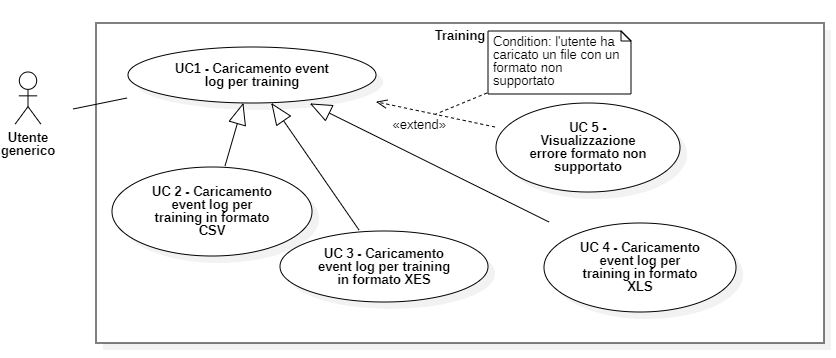
\includegraphics[scale=0.6]{immagini/usecase/cd1.JPG}
    \caption{Casi d'uso relativi al caricamento file di training}
\end{figure}

\subsubsection{UC 1 - Caricamento dell'event log per il training}
\begin{itemize}
	\item \textbf{Attore primario:} Utente generico;
	\item \textbf{Descrizione:} L'utente deve poter caricare l'event log per la fase di training;
	\item \textbf{Scenario principale:} 
		\begin{enumerate}
			\item L'utente seleziona l'event log su cui eseguire il training, in formato CSV (\textbf{UC 2}), XES (\textbf{UC 3}) o XLS (\textbf{UC 4});
			\item L'utente carica l'event log.
		\end{enumerate}
	\item \textbf{Estensioni:} L'utente ha tentato di caricare un event log con formato non supportato e viene mostrato un errore (\textbf{UC 4});
	\item \textbf{Precondizioni:} Non è stato caricato nessun event log su cui effettuare training;
	\item \textbf{Postcondizioni:} L'event log per il training è stato correttamente caricato nel sistema.

\end{itemize}

\subsubsection{UC 2 - Caricamento dell'event log per il training in formato CSV}
\begin{itemize}
	\item \textbf{Attore primario:} Utente generico;
	\item \textbf{Descrizione:} L'utente deve poter caricare l'event log per il training in formato CSV;
	\item \textbf{Scenario principale:} L'utente carica l'event log per il training in formato CSV;
	\item \textbf{Precondizioni:} Non è stato caricato nessun event log su cui effettuare training;
	\item \textbf{Postcondizioni:} L'event log per il training in formato CSV è stato correttamente caricato nel sistema.

\end{itemize}

\subsubsection{UC 3 - Caricamento dell'event log per il training in formato XES}
\begin{itemize}

	\item \textbf{Attore primario:} Utente generico;
	\item \textbf{Descrizione:} L'utente deve poter caricare l'event log per il training in formato XES;
	\item \textbf{Scenario principale:} L'utente carica l'event log per il training in formato XES;
	\item \textbf{Precondizioni:} Non è stato caricato nessun event log su cui effettuare training;
	\item \textbf{Postcondizioni:} L'event log per il training in formato XES è stato correttamente caricato nel sistema.

\end{itemize}



\subsubsection{UC 4 - Caricamento dell'event log per il training in formato XLS}
\begin{itemize}
	\item \textbf{Attore primario:} Utente generico;
	\item \textbf{Descrizione:} L'utente deve poter caricare l'event log per il training in formato XLS;
	\item \textbf{Scenario principale:} L'utente carica l'event log per il training in formato XLS;
	\item \textbf{Precondizioni:} Non è stato caricato nessun event log su cui effettuare training;
	\item \textbf{Postcondizioni:} L'event log per il training in formato XLS è stato correttamente caricato nel sistema.

\end{itemize}



\subsubsection{UC 5 - Visualizzazione errore formato non supportato}
\begin{itemize}
	\item \textbf{Attore primario:} Utente generico;
	\item \textbf{Descrizione:} L'utente deve ricevere un errore in caso venga caricato un event log con formato non supportato
	\item \textbf{Scenario principale:} 
		\begin{enumerate}
			\item L'utente seleziona un event log da caricare con un formato non supportato;
			\item L'utente carica l'event log;
			\item Viene mostrato un messaggio d'errore esplicativo.
		\end{enumerate}
	
	\item \textbf{Precondizioni:} L'utente ha caricato un event log con un formato non supportato;
	\item \textbf{Postcondizioni:} Viene mostrato il messaggio d'errore e l'event log non viene caricato.
\end{itemize}



\begin{figure}[H]
    \centering
    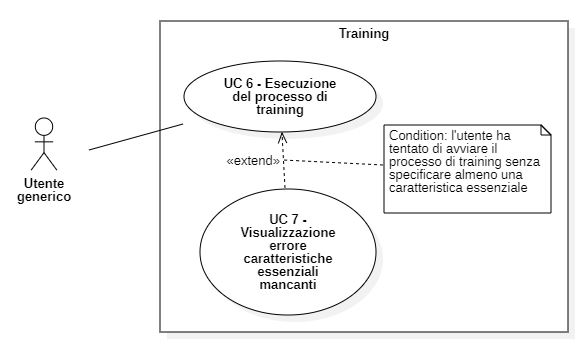
\includegraphics[scale=0.6]{immagini/usecase/cd2.JPG}
    \caption{Casi d'uso relativi al processo di training}
\end{figure}

\subsubsection{UC 6 - Esecuzione del processo di training}
\begin{itemize}
	\item \textbf{Attore primario:} Utente generico;
	\item \textbf{Descrizione:} L'utente deve poter avviare il processo di training;
	\item \textbf{Scenario principale:} 
		\begin{enumerate}
			\item L'utente seleziona le colonne relative alle features dell'event log (\textbf{UC 6.1});
			\item L'utente seleziona il KPI che desidera (\textbf{UC 6.2});		
			\item L'utente seleziona la soglia di frequenza degli outliers che desidera (\textbf{UC 6.3});
			\item L'utente clicca sul pulsante "Start training";
			\item Il processo di training sull'event log caricato e con le caratteristiche selezionate viene avviato:
			\item L'utente visualizza il progresso del processo di training (\textbf{UC 6.4}); 
			\item Al termine del processo l'utente viene notificato;
		\end{enumerate}
	\item \textbf{Estensioni:} Almeno una delle caratteristiche necessarie non è stata specificata e viene mostrato un errore all'utente (\textbf{UC 7});
	\item \textbf{Precondizioni:} L'event log per il training è stato caricato correttamente (\textbf{UC 1});
	\item \textbf{Postcondizioni:} Il processo di training è stato completato con successo. 

\end{itemize}


\begin{figure}[H]
    \centering
    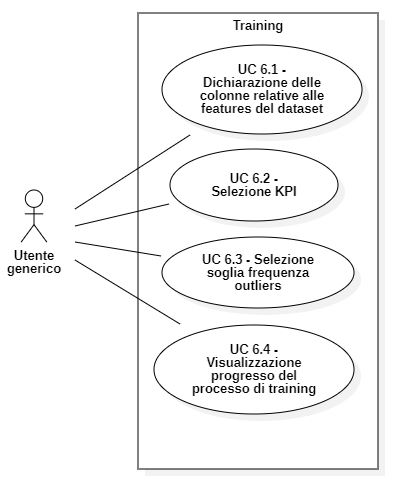
\includegraphics[scale=0.6]{immagini/usecase/cd3.JPG}
    \caption{Casi d'uso relativi al processo di training}
\end{figure}

\subsubsection{UC 6.1 - Dichiarazione delle colonne relative alle features del dataset}
\begin{itemize}
	\item \textbf{Attore primario:} Utente generico;
	\item \textbf{Descrizione:} L'utente deve poter dichiarare quali colonne sono relative a quali features del dataset caricato.
	\item \textbf{Scenario principale:} 
		\begin{enumerate}
			\item L'utente dichiara la colonna relativa alla feature "id" (\textbf{UC 6.1.1});
			\item L'utente dichiara la colonna relativa alla feature "activity" (\textbf{UC 6.1.2});
			\item L'utente dichiara la colonna relativa alla feature "timestamp" (\textbf{UC 6.1.3});
			\item L'utente dichiara la colonna relativa alla feature "resurce" (\textbf{UC 6.1.4}).
		\end{enumerate}
	
	\item \textbf{Precondizioni:} L'event log in formato CSV o XLS è stato caricato correttamente (\textbf{UC 2}, \textbf{UC 4});
	\item \textbf{Postcondizioni:} Il sistema conosce a quale colonna corrisponde ogni feature relative al dataset CSV o XLS caricato.
\end{itemize}

\begin{figure}[H]
    \centering
    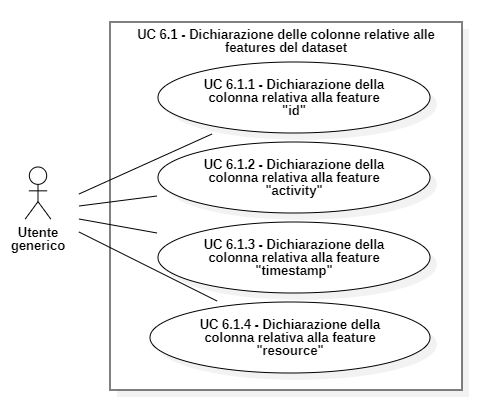
\includegraphics[scale=0.6]{immagini/usecase/cd5.JPG}
    \caption{Casi d'uso relativi alla dichiarazione delle colonne}
\end{figure}

\subsubsection{UC 6.1.1 - Dichiarazione della colonna relativa alla feature "id"}
\begin{itemize}
	\item \textbf{Attore primario:} Utente generico;
	\item \textbf{Descrizione:} L'utente deve poter selezionare la colonna corrispondente alla feature "id".
	\item \textbf{Scenario principale:} 
		\begin{enumerate}
			\item L'utente seleziona il campo relativo alla feature "id";
			\item L'utente dichiara la colonna relativa alla feature "id".
		\end{enumerate}
	\item \textbf{Precondizioni:} L'event log in formato CSV o XLS è stato caricato correttamente (\textbf{UC 2}, \textbf{UC 4});
	\item \textbf{Postcondizioni:} La colonna relativa alla feature "id" è stata dichiarata.
\end{itemize}


\subsubsection{UC 6.1.2 - Dichiarazione della colonna relativa alla feature "activity"}
\begin{itemize}
	\item \textbf{Attore primario:} Utente generico;
	\item \textbf{Descrizione:} L'utente deve poter selezionare la colonna corrispondente alla feature "activity".
	\item \textbf{Scenario principale:} 
		\begin{enumerate}
			\item L'utente seleziona il campo relativo alla feature "activity";
			\item L'utente dichiara la colonna relativa alla feature "activity".
		\end{enumerate}
	\item \textbf{Precondizioni:}  L'event log in formato CSV o XLS è stato caricato correttamente (\textbf{UC 2}, \textbf{UC 4});
	\item \textbf{Postcondizioni:} La colonna relativa alla feature "activity" è stata dichiarata.
\end{itemize}

\subsubsection{UC 6.1.3 - Dichiarazione della colonna relativa alla feature "timestamp"}
\begin{itemize}
	\item \textbf{Attore primario:} Utente generico;
	\item \textbf{Descrizione:} L'utente deve poter selezionare la colonna corrispondente alla feature "timestamp".
	\item \textbf{Scenario principale:} 
		\begin{enumerate}
			\item L'utente seleziona il campo relativo alla feature "timestamp";
			\item L'utente dichiara la colonna relativa alla feature "timestamp".
		\end{enumerate}
	\item \textbf{Precondizioni:}  L'event log in formato CSV o XLS è stato caricato correttamente (\textbf{UC 2}, \textbf{UC 4});
	\item \textbf{Postcondizioni:} La colonna relativa alla feature "timestamp" è stata dichiarata.
\end{itemize}

\subsubsection{UC 6.1.4 - Dichiarazione della colonna relativa alla feature "resource"}
\begin{itemize}
	\item \textbf{Attore primario:} Utente generico;
	\item \textbf{Descrizione:} L'utente deve poter selezionare la colonna corrispondente alla feature "resource".
	\item \textbf{Scenario principale:} 
		\begin{enumerate}
			\item L'utente seleziona il campo relativo alla feature "resource";
			\item L'utente dichiara la colonna relativa alla feature "resource".
		\end{enumerate}
	\item \textbf{Precondizioni:}  L'event log in formato CSV o XLS è stato caricato correttamente (\textbf{UC 2}, \textbf{UC 4});
	\item \textbf{Postcondizioni:} La colonna relativa alla feature "resource" è stata dichiarata.
\end{itemize}


\subsubsection{UC 6.2 - Selezione KPI}
\begin{itemize}
	\item \textbf{Attore primario:} Utente generico;
	\item \textbf{Descrizione:} L'utente deve poter selezionare il KPI che desidera tra quelli disponibili;
	\item \textbf{Scenario principale:} L'utente seleziona il KPI tra:
		\begin{itemize}
			\item "Total time" (\textbf{UC 6.2.1});
			\item "Minimize activity occurence" (\textbf{UC 6.2.2});
			%\item "Maximize activity occurence" (\textbf{UC 5.1.3});
			%\item "Cost" (\textbf{UC 5.3});
		\end{itemize}
	\item \textbf{Precondizioni:} Il file di training è stato caricato correttamente (\textbf{UC 1});
	\item \textbf{Postcondizioni:} Il KPI è stato selezionato.
\end{itemize}

\begin{figure}[H]
    \centering
    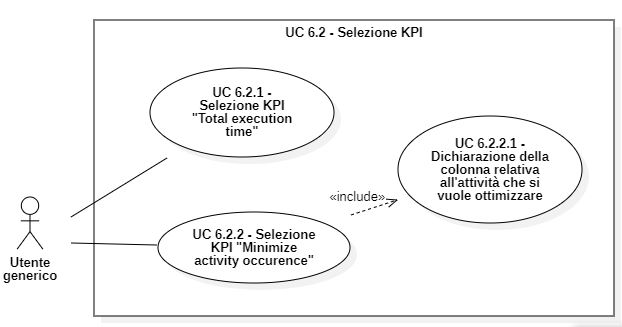
\includegraphics[scale=0.6]{immagini/usecase/cd4.JPG}
    \caption{Casi d'uso relativi alla selezione del KPI}
\end{figure}

\subsubsection{UC 6.2.1 - Selezione KPI "Total time"}
\begin{itemize}
	\item \textbf{Attore primario:} Utente generico;
	\item \textbf{Descrizione:} L'utente deve poter selezionare il KPI "Total time";
	\item \textbf{Scenario principale:} L'utente seleziona il KPI "Total time";
			
	\item \textbf{Precondizioni:} Il file di training è stato caricato correttamente (\textbf{UC 1});
	\item \textbf{Postcondizioni:} Il KPI "Total time" è stato selezionato.
\end{itemize}

%\subsubsection{UC 5.1.2 - Selezione KPI "Maximize activity occurence"}
%\begin{itemize}
%	\item \textbf{Attore primario:} Utente generico;
%	\item \textbf{Descrizione:} L'utente deve poter selezionare il KPI "Maximize activity occurence";
%	\item \textbf{Scenario principale:}
%		\begin{enumerate}
%			\item L'utente seleziona il KPI "Maximize activity occurence";
%			\item L'utente dichiara la colonna relativa all'attività di cui vuole massimizzare le occorrenze (\textbf{UC 5.1.2.1}).
%		\end{enumerate}
%			
%	\item \textbf{Precondizioni:} Il file di training è stato caricato correttamente (\textbf{UC 1});
%	\item \textbf{Postcondizioni:} Il KPI "Maximize activity occurence" è stato selezionato.
%\end{itemize}

\subsubsection{UC 6.2.2 - Selezione KPI "Minimize activity occurence"}
\begin{itemize}
	\item \textbf{Attore primario:} Utente generico;
	\item \textbf{Descrizione:} L'utente deve poter selezionare il KPI "Minimize activity occurence";
	\item \textbf{Scenario principale:}
		\begin{enumerate}
			\item L'utente seleziona il KPI "Minimize activity occurence";
			\item L'utente dichiara la colonna relativa all'attività di cui vuole minimizzare le occorrenze (\textbf{UC 6.2.2.1}).
		\end{enumerate}
			
	\item \textbf{Precondizioni:} Il file di training è stato caricato correttamente (\textbf{UC 1});
	\item \textbf{Postcondizioni:} Il KPI "Minimize activity occurence" è stato selezionato.
\end{itemize}

%\subsubsection{UC 5.3 - Selezione KPI "Cost"}
%\begin{itemize}
%	\item \textbf{Attore primario:} Utente generico;
%	\item \textbf{Descrizione:} L'utente deve poter selezionare il KPI "Cost";
%	\item \textbf{Scenario principale:} L'utente seleziona il KPI "Cost";
%			
%	\item \textbf{Precondizioni:} Il file di training è stato caricato correttamente (\textbf{UC 1});
%	\item \textbf{Postcondizioni:} Il KPI "Cost" è stato selezionato.
%\end{itemize}


\subsubsection{UC 6.2.2.1 - Dichiarazione della colonna relativa all'attività che si vuole ottimizzare}
\begin{itemize}
	\item \textbf{Attore primario:} Utente generico;
	\item \textbf{Descrizione:} L'utente deve poter selezionare la colonna corrispondente all'attività che vuole ottimizzare;
	\item \textbf{Scenario principale:} 
		\begin{enumerate}
			\item L'utente seleziona il campo relativo all'attività che vuole ottimizzare;
			\item L'utente dichiara la colonna relativa all'attività che vuole ottimizzare.
		\end{enumerate}
	\item \textbf{Precondizioni:} 
		\begin{itemize}
			\item Il KPI "Minimize activity occurence" è stato selezionato (\textbf{UC 6.1.3});
			\item La feature "activity" è stata selezionata (\textbf{UC 6.1.2});
		\end{itemize}			
	
	
	\item \textbf{Postcondizioni:} L'attività che si vuole ottimizzare è stata dichiarata.
\end{itemize}


\subsubsection{UC 6.3 - Selezione soglia frequenza outliers}
\begin{itemize}
	\item \textbf{Attore primario:} Utente generico;
	\item \textbf{Descrizione:} L'utente deve avere la possibilità di selezionare la soglia della frequenza degli outliers che desidera;
	\item \textbf{Scenario principale:} L'utente seleziona la soglia che desidera;
	\item \textbf{Estensioni:} Se l'utente non seleziona nessuna soglia viene considerata una soglia di default;
	\item \textbf{Precondizioni:} L'utente ha caricato correttamente il file di training (UC 1);
	\item \textbf{Postcondizioni:} La soglia immessa è stata registrata dal sistema.
\end{itemize}





\subsubsection{UC 6.4 - Visualizzazione progresso del processo di training}
\begin{itemize}
	\item \textbf{Attore primario:} Utente generico;
	\item \textbf{Descrizione:} L'utente deve poter visualizzazione il progresso del processo di training
	\item \textbf{Scenario principale:} L'utente visualizza un indicatore relativo all'attuale progresso del processo di training;
	\item \textbf{Precondizioni:} Il processo di training è stato avviato correttamente (\textbf{UC 6});
	\item \textbf{Postcondizioni:} L'utente è in grado di stimare quanto manca al termine del processo di training.
\end{itemize}


\subsubsection{UC 7 - Visualizzazione errore caratteristiche essenziali mancanti}
\begin{itemize}
	\item \textbf{Attore primario:} Utente generico;
	\item \textbf{Descrizione:} L'utente ha tentanto di avviare il training non avendo inserito una delle caratteristiche essenziali;
	\item \textbf{Scenario principale:}
		\begin{enumerate}
			\item L'utente non ha specificato almeno una tra le seguenti caratteristiche essenziali:
				\begin{itemize}
					\item KPI (\textbf{UC 6.2});
					\item Colonna relativa ad una feature (\textbf{UC 6.1.x});
					\item Attività da ottimizzare (\textbf{UC 6.2.2.1}).
				\end{itemize}
			\item L'utente ha cliccato il pulsante "Start training";
			
		\end{enumerate}
	\item \textbf{Precondizioni:} L'utente ha tentato di avviare il processo di training senza specificare almeno una caratteristica essenziale; 
	\item \textbf{Postcondizioni:} Il processo di training non viene avviato e all'utente viene visualizzato un errore esplicativo.
\end{itemize}


\subsubsection{UC 8 - Download del process model generato dal processo di training}
\begin{itemize}
	\item \textbf{Attore primario:} Utente generico;
	\item \textbf{Descrizione:} L'utente deve poter fare il download dei file del process model generato del processo di training;
	\item \textbf{Scenario principale:}
		\begin{enumerate}
			\item L'utente clicca il pulsante "Download training files";
			\item I file che compongono il process model vengono scaricati.
		\end{enumerate}
	\item \textbf{Precondizioni:} L'utente ha terminato con successo il processo di training (\textbf{UC 6}); 
	\item \textbf{Postcondizioni:} L'utente ha scaricato i file del process model.
\end{itemize}



%% -------------------------
%% ---- RUNNING PHASE ------
%% -------------------------

\begin{figure}[H]
    \centering
    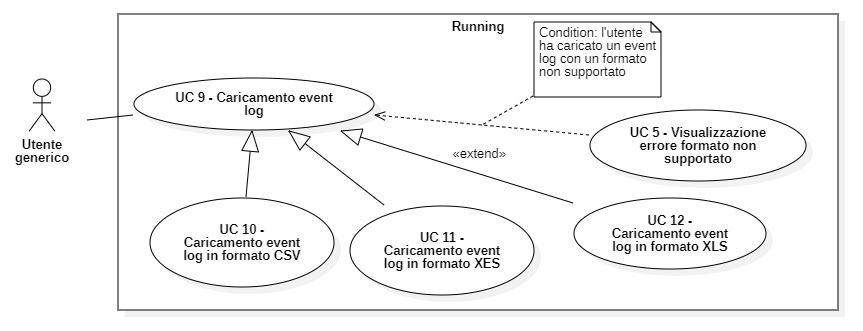
\includegraphics[scale=0.6]{immagini/usecase/cd6.JPG}
    \caption{Casi d'uso relativi al caricamento del file di log}
\end{figure}


\subsubsection{UC 9 - Caricamento dell'event log per il calcolo delle raccomandazioni}
\begin{itemize}
	\item \textbf{Attore primario:} Utente generico;
	\item \textbf{Descrizione:} L'utente deve poter caricare l'event log per il calcolo delle raccomandazioni;
	\item \textbf{Scenario principale:} 
		\begin{enumerate}
			\item L'utente seleziona l'event log per il calcolo delle raccomandazioni in formato CSV (\textbf{UC 10}), XES (\textbf{UC 11}) o XLS (\textbf{UC 12});
			\item L'utente carica l'event log selezionato.
		\end{enumerate}
	\item \textbf{Estensioni:} L'utente ha tentato di caricare un event log con formato non supportato e viene mostrato un errore (\textbf{UC 5});
		
	\item \textbf{Precondizioni:} La fase di training è stata completata (\textbf{UC 6}) oppure l'utente ha caricato un modello già allenato (\textbf{UC 19});
	\item \textbf{Postcondizioni:} L'event log per la running phase è stato correttamente caricato nel sistema.
\end{itemize}

\subsubsection{UC 10 - Caricamento dell'event log per il calcolo delle raccomandazioni in formato CSV}
\begin{itemize}
	\item \textbf{Attore primario:} Utente generico;
	\item \textbf{Descrizione:} L'utente deve poter caricare l'event log per il calcolo delle raccomandazioni in formato CSV;
	\item \textbf{Scenario principale:} L'utente carica l'event log per il calcolo delle raccomandazioni in formato CSV;
	\item \textbf{Precondizioni:} Non è stato caricato nessun event log per il calcolo delle raccomandazioni;
	\item \textbf{Postcondizioni:} L'event log per il calcolo delle raccomandazioni in formato XES è stato correttamente caricato nel sistema.
\end{itemize}

\subsubsection{UC 11 - Caricamento dell'event log per il calcolo delle raccomandazioni in formato XES}
\begin{itemize}
	\item \textbf{Attore primario:} Utente generico;
	\item \textbf{Descrizione:} L'utente deve poter caricare l'event log per il calcolo delle raccomandazioni in formato XES;
	\item \textbf{Scenario principale:} L'utente carica l'event log per il calcolo delle raccomandazioni in formato XES;
	\item \textbf{Precondizioni:} Non è stato caricato nessun event log per il calcolo delle raccomandazioni;
	\item \textbf{Postcondizioni:} L'event log per il calcolo delle raccomandazioni in formato XES è stato correttamente caricato nel sistema.
\end{itemize}

\subsubsection{UC 12 - Caricamento dell'event log per il calcolo delle raccomandazioni in formato XLS}
\begin{itemize}
	\item \textbf{Attore primario:} Utente generico;
	\item \textbf{Descrizione:} L'utente deve poter caricare l'event log per il calcolo delle raccomandazioni in formato XLS;
	\item \textbf{Scenario principale:} L'utente carica l'event log per il calcolo delle raccomandazioni in formato XLS;
	\item \textbf{Precondizioni:} Non è stato caricato nessun event log per il calcolo delle raccomandazioni;
	\item \textbf{Postcondizioni:} L'event log per il calcolo delle raccomandazioni in formato XLS è stato correttamente caricato nel sistema.
\end{itemize}

\begin{figure}[H]
    \centering
    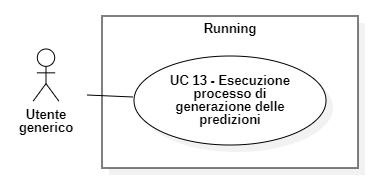
\includegraphics[scale=0.6]{immagini/usecase/cd7.JPG}
    \caption{Caso d'uso relativo al processo di generazione delle raccomandazioni}
\end{figure}

\subsubsection{UC 13 - Esecuzione processo di generazione delle raccomandazioni}
\begin{itemize}
	\item \textbf{Attore primario:} Utente generico;
	\item \textbf{Descrizione:} L'utente deve poter avviare il processo di generazione delle raccomandazioni;
	\item \textbf{Scenario principale:} 
		\begin{enumerate}
			\item L'utente clicca sul pulsante "Generate recommendations";
			\item Il processo di generazione delle predizioni sull'event log caricato si avvia;
			\item L'utente visualizza il progresso del processo di generazione delle raccomandazioni (\textbf{UC 13.1});
			\item Al termine del processo l'utente viene notificato.
		\end{enumerate}
	\item \textbf{Precondizioni:} L'event log per il calcolo delle raccomandazioni è stato caricato correttamente (\textbf{UC 9});
	\item \textbf{Postcondizioni:} Il processo di generazione delle raccomandazioni è stato completato con successo. 
\end{itemize}

\begin{figure}[H]
    \centering
    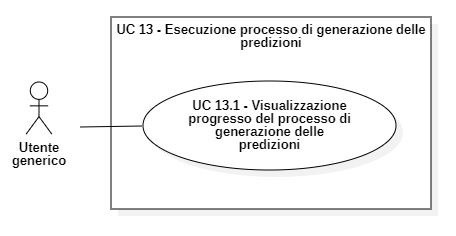
\includegraphics[scale=0.6]{immagini/usecase/cd8.JPG}
    \caption{Caso d'uso relativo alla visualizzazione del progresso relativo al processo di generazione delle raccomandazioni}
\end{figure}

\subsubsection{UC 13.1 - Visualizzazione progresso del processo di generazione delle raccomandazioni}
\begin{itemize}
	\item \textbf{Attore primario:} Utente generico;
	\item \textbf{Descrizione:} L'utente deve poter visualizzazione il progresso del processo di generazione delle raccomandazioni
	\item \textbf{Scenario principale:} L'utente visualizza un indicatore relativo all'attuale progresso del processo di generazione delle raccomandazioni;
	\item \textbf{Precondizioni:} Il processo di generazione delle raccomandazioni è stato avviato correttamente (\textbf{UC 13});
	\item \textbf{Postcondizioni:} L'utente è in grado di stimare quanto manca al termine del processo di generazione delle raccomandazioni.
\end{itemize}

\begin{figure}[H]
    \centering
    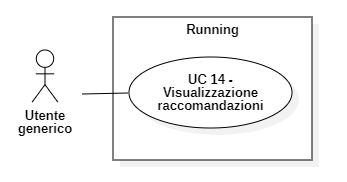
\includegraphics[scale=0.6]{immagini/usecase/cd9.JPG}
    \caption{Caso d'uso relativo alla visualizzazione delle raccomandazioni}
\end{figure}

\subsubsection{UC 14 - Visualizzazione raccomandazioni}
\begin{itemize}
	\item \textbf{Attore primario:} Utente generico;
	\item \textbf{Descrizione:} L'utente deve essere in grado di visualizzare le raccomandazioni generate;
	\item \textbf{Scenario principale:} L'utente visualizza l'insieme delle raccomandazioni generate.

	\item \textbf{Sottocasi:}
		\begin{itemize}
			\item L'utente visualizza la raccomandazione relativa alla singola traccia (\textbf{UC 14.1});
		\end{itemize}
		
	\item \textbf{Estensioni:} L'utente può riordinare le raccomandazioni secondo alcuni ordinamenti predefiniti (\textbf{UC 14.2})
	\item \textbf{Precondizioni:} Il processo di generazione delle predizioni è completato (\textbf{UC 13});
	\item \textbf{Postcondizioni:} L'utente ha visualizzato le predizioni.
\end{itemize}

\begin{figure}[H]
    \centering
    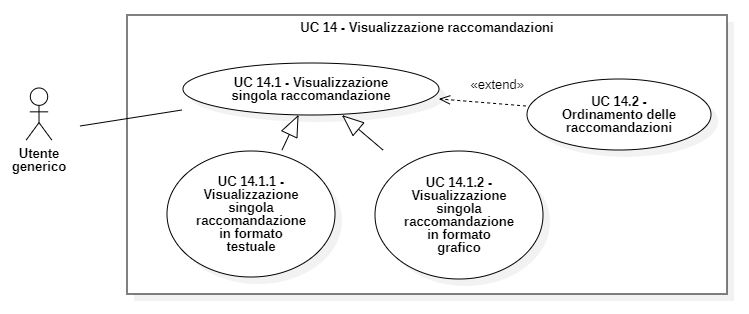
\includegraphics[scale=0.6]{immagini/usecase/cd10.JPG}
    \caption{Casi d'uso relativi alla visualizzazione della singola raccomandazione}
\end{figure}

\subsubsection{UC 14.1 - Visualizzazione raccomandazioni per una singola traccia}
\begin{itemize}
	\item \textbf{Attore primario:} Utente generico;
	\item \textbf{Descrizione:} L'utente deve poter visualizzare le raccomandazioni per una singola traccia;
	\item \textbf{Scenario principale:}
		\begin{enumerate}
			\item L'utente seleziona la traccia a cui è interessato;
			\item L'utente visualizza le raccomandazioni (per la singola traccia) in formato testuale (\textbf{UC 14.1.1}) e grafico (\textbf{UC 14.1.2}).
		\end{enumerate}
	\item \textbf{Precondizioni:} L'utente sta svolgendo l'attività di visualizzazione;
	\item \textbf{Postcondizioni:} L'utente ha visualizzato le raccomandazioni di suo interesse.
\end{itemize}

\subsubsection{UC 14.1.1 - Visualizzazione singola raccomandazione in formato testuale}
\begin{itemize}
	\item \textbf{Attore primario:} Utente generico;
	\item \textbf{Descrizione:} L'utente deve poter visualizzare le migliori raccomandazioni (fino ad un massimo di 3) e la predizione dell'attività in corso, con i corrispettivi KPI espressi in maniera testuale;
	\item \textbf{Scenario principale:}
		\begin{enumerate}
			\item L'utente visualizza le 3 migliori raccomandazioni e la predizione dell'attività in corso; 
			\item L'utente visualizza i KPI predetti delle attività raccomandate e visualizza il KPI della predizione sulla base dell'attività in corso.
		\end{enumerate}
	\item \textbf{Precondizioni:} L'utente sta svolgendo l'attività di visualizzazione;
	\item \textbf{Postcondizioni:} L'utente ha visualizzato la singola raccomandazione di suo interesse.
\end{itemize}

\subsubsection{UC 14.1.2 - Visualizzazione singola raccomandazione in formato grafico}
\begin{itemize}
	\item \textbf{Attore primario:} Utente generico;
	\item \textbf{Descrizione:} L'utente deve poter visualizzare i KPI della migliore raccomandazione in forma grafica;
	\item \textbf{Scenario principale:} L'utente visualizza un grafico che rappresenta i KPI della migliore attività raccomandata;
	\item \textbf{Precondizioni:} L'utente sta svolgendo l'attività di visualizzazione;
	\item \textbf{Postcondizioni:} L'utente ha visualizzato la singola predizione di suo interesse tramite un grafico.
\end{itemize}


\subsubsection{UC 14.2 - Ordinamento delle raccomandazioni}
\begin{itemize}
	\item \textbf{Attore primario:} Utente generico;
	\item \textbf{Descrizione:} L'utente può riordinare l'insieme di tutte le raccomandazioni secondo alcuni ordinamenti predefiniti;
	\item \textbf{Scenario principale:} 
	\begin{itemize}
		\item L'utente sceglie in tipo di ordinamento tra:
			\begin{itemize}
				\item "Delta from maximum": Le raccomandazioni sono riordinate in ordine decrescente di variazione;
				\item "Delta from minimum": Le raccomandazioni sono riordinate in ordine crescente di variazione;
				\item "Maximize": Le raccomandazioni sono riordinate in ordine decrescente; 
				\item "Minimize": Le raccomandazioni sono riordinate in ordine crescente;
			\end{itemize}
		\item L'utente visualizza le raccomandazioni con il nuovo ordinamento;
	\end{itemize}
	\item \textbf{Precondizioni:} L'utente sta visualizzando tutte le raccomandazioni generate;
	\item \textbf{Postcondizioni:} L'utente visualizza le raccomandazioni riordinate secondo l'ordinamento scelto;
\end{itemize}

\subsubsection{UC 15 - Ricerca traccia per id}
\begin{itemize}
	\item \textbf{Attore primario:} Utente generico;
	\item \textbf{Descrizione:} L'utente deve poter ricercare le tracce per id
	\item \textbf{Scenario principale:} 
		\begin{enumerate}
			\item L'utente seleziona il campo di ricerca;
			\item L'utente digita l'id della traccia a cui è interessato;
			\item L'utente può selezionare la traccia ricercata;
		\end{enumerate}
	\item \textbf{Precondizioni:} L'utente sta svolgendo l'attività di ricerca;
	\item \textbf{Postcondizioni:} L'utente ha trovato la traccia corrispondente all'id a cui era interessato.
\end{itemize}

\subsubsection{UC 16 - Ricerca traccia tramite grafico}
\begin{itemize}
	\item \textbf{Attore primario:} Utente generico;
	\item \textbf{Descrizione:} L'utente deve poter ricercare le tracce selezionandole in un grafico che le rappresenta; 
	\item \textbf{Scenario principale:} 
		\begin{enumerate}
			\item L'utente visualizza un grafico che mostra tutte le tracce;
			\item L'utente clicca sulla traccia a cui è interessato;
			\item La traccia viene selezionata;
		\end{enumerate}
	\item \textbf{Precondizioni:} L'utente sta svolgendo l'attività di ricerca;
	\item \textbf{Postcondizioni:} L'utente ha selezionato una traccia a cui è interessato.
\end{itemize}

\begin{figure}[H]
    \centering
    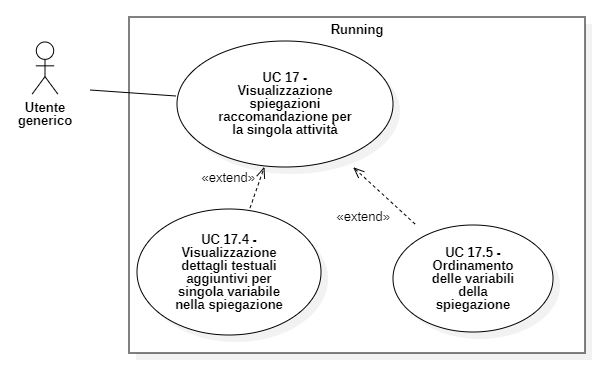
\includegraphics[scale=0.6]{immagini/usecase/cd11.JPG}
    \caption{Caso d'uso relativo alla visualizzazione delle spiegazioni}
\end{figure}

\subsubsection{UC 17 - Visualizzazione spiegazioni singola raccomandazione}
\begin{itemize}
	\item \textbf{Attore primario:} Utente generico;
	\item \textbf{Descrizione:} L'utente deve poter visualizzare le spiegazioni per ogni raccomandazione di una singola traccia
	\item \textbf{Scenario principale:} 
		\begin{enumerate}
			\item L'utente seleziona la traccia a cui è interessato (\textbf{UC 15}, \textbf{UC 16});
			\item L'utente seleziona la raccomandazione di cui vuole visualizzare la spiegazione (\textbf{UC 17.1});
			\item L'utente seleziona la quantità di variabili che vuole visualizzare nella spiegazione(\textbf{UC 17.2});
			\item L'utente visualizza la spiegazione in formato grafico (\textbf{UC 17.3}); 
		\end{enumerate}
	\item \textbf{Estensioni}: 
	\begin{itemize}
		\item Una volta visualizzate le spiegazioni l'utente può selezionare una singola variabile spiegata per poter ottenere dettagli testuali aggiuntivi (\textbf{UC 17.4});
		\item L'utente può riordinare le variabili delle spiegazioni secondo ordinamenti predefiniti (\textbf{17.5});
	\end{itemize}

	\item \textbf{Precondizioni:} L'utente sta svolgendo l'attività di visualizzazione e il processo di generazione delle raccomandazioni è completato (\textbf{UC 13});
	\item \textbf{Postcondizioni:} L'utente ha visualizzato le spiegazioni relative ad una attività tra quelle raccomandate per una traccia di suo interesse.
\end{itemize}

\begin{figure}[H]
    \centering
    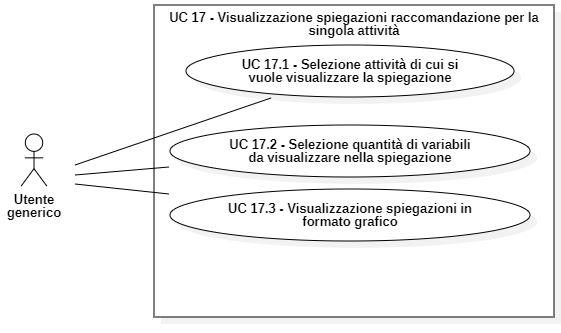
\includegraphics[scale=0.6]{immagini/usecase/cd12.JPG}
    \caption{Casi d'uso relativi alla visualizzazione di una singola raccomandazione}
\end{figure}

\subsubsection{UC 17.1 - Selezione attività di cui si vuole visualizzare la spiegazione}
\begin{itemize}
	\item \textbf{Attore primario:} Utente generico;
	\item \textbf{Descrizione:} L'utente deve poter selezionare l'attività raccomandata di cui vuole visualizzare la spiegazione;
	\item \textbf{Scenario principale:} L'utente seleziona l'attività raccomandata che desidera;

	\item \textbf{Precondizioni:} L'utente sta svolgendo l'attività di visualizzazione delle raccomandazioni;
	\item \textbf{Postcondizioni:} Il sistema ha registrato l'attività a cui l'utente è interessato di vedere le spiegazioni.
\end{itemize}

\subsubsection{UC 17.2 - Selezione quantità di variabili da visualizzare nella spiegazione}
\begin{itemize}
	\item \textbf{Attore primario:} Utente generico;
	\item \textbf{Descrizione:} L'utente deve poter visualizzare quante variabili visualizzare per la spiegazione;
	\item \textbf{Scenario principale:}
	\begin{enumerate}
			\item L'utente seleziona il campo di selezione quantità;
			\item L'utente sceglie la quantità desiderata.
		\end{enumerate}
	
	\item \textbf{Precondizioni:} L'utente sta svolgendo l'attività di visualizzazione delle raccomandazioni;
	\item \textbf{Postcondizioni:} Il sistema ha registrato la quantità di spiegazione che l'utente è interessato a visualizzare
\end{itemize}

\subsubsection{UC 17.3 - Visualizzazione spiegazione in formato grafico}
\begin{itemize}
	\item \textbf{Attore primario:} Utente generico;
	\item \textbf{Descrizione:} L'utente deve poter visualizzare un grafico che rappresenta le singole variazioni relative alle variabili da spiegare;
	\item \textbf{Scenario principale:} L'utente visualizza un grafico in cui sono rappresentati le singole variazioni alle variabili prese in considerazione;
	
	\item \textbf{Precondizioni:}
	\begin{itemize}
			\item l'utente ha selezionato l'attività di cui vuole visualizzare la spiegazione (\textbf{UC 17.1}) 
	 		\item l'utente ha selezionato la quantità di variabili che desidera visualizzare nella spiegazione 	(\textbf{UC 17.2})
	 	\end{itemize}
	\item \textbf{Postcondizioni:} L'utente ha visualizzato le spiegazione in formato grafico;
\end{itemize}


\subsubsection{UC 17.4 - Visualizzazione dettagli testuali aggiuntivi per singola variabile nella spiegazione}
\begin{itemize}
	\item \textbf{Attore primario:} Utente generico;
	\item \textbf{Descrizione:} L'utente può selezionare una singola variabile per ottenere una spiegazione testuale più dettagliata;
	\item \textbf{Scenario principale:} 
		\begin{itemize}
			\item L'utente seleziona la variabile della spiegazione sui cui vuole avere dei dettagli aggiuntivi;
			\item L'utente visualizza i dettagli aggiuntivi relativi alla variabile selezionata in forma testuale;
		\end{itemize}
	
	\item \textbf{Precondizioni:} L'utente sta visualizzando la spiegazione di una raccomandazione;
	\item \textbf{Postcondizioni:} L'utente ha ottenuto dettaglia aggiuntivi su una singola variabile della spiegazione;
\end{itemize}

\subsubsection{UC 17.5 - Ordinamento delle variabili della spiegazione}
\begin{itemize}
	\item \textbf{Attore primario:} Utente generico;
	\item \textbf{Descrizione:} L'utente può riordinare le variabili della spiegazione secondo alcuni ordinamenti predefiniti;
	\item \textbf{Scenario principale:} 
	\begin{itemize}
		\item L'utente sceglie in tipo di ordinamento tra:
			\begin{itemize}
				\item "Delta from maximum": Le variabili della spiegazione sono riordinate in ordine decrescente di variazione;
				\item "Delta from minimum": Le variabili della spiegazione sono riordinate in ordine crescente di variazione;
			\end{itemize}
		\item L'utente visualizza le spiegazioni con il nuovo ordinamento;
	\end{itemize}
	\item \textbf{Precondizioni:} L'utente sta visualizzando la spiegazione di una raccomandazione;
	\item \textbf{Postcondizioni:} L'utente visualizza le variabili della spiegazione riordinate secondo l'ordinamento scelto;
\end{itemize}


\subsubsection{UC 18 - Inserimento nome esperimento}
\begin{itemize}
	\item \textbf{Attore primario:} Utente generico;
	\item \textbf{Descrizione:} L'utente deve poter nominare l'esperimento effettuato;
	\item \textbf{Scenario principale:} L'utente inserisce il nome che preferisce per l'esperimento;
	\item \textbf{Estensioni:} Se l'utente non inserisce nessun nome viene inserito un nome di default; 
	\item \textbf{Precondizioni:} L'utente non ha ancora iniziato il processo di training (\textbf{UC 6})
	\item \textbf{Postcondizioni:} Il sistema ha registrato la preferenza dell'utente.
\end{itemize}

\subsubsection{UC 19 - Caricamento modello già precedentemente allenato}
\begin{itemize}
	\item \textbf{Attore primario:} Utente generico;
	\item \textbf{Descrizione:} L'utente deve poter caricare un modello già allenato (permettendo di saltare la fase di training)
	\item \textbf{Scenario principale:}
		\begin{enumerate}
			\item L'utente seleziona il campo relativo al caricamento di modelli già allenati;
			\item L'utente seleziona un modello da caricare;
			\item L'utente clicca su "Load model".
		\end{enumerate}
	\item \textbf{Precondizioni:} L'utente deve aver a disposizione dei modelli già allenati; 
	\item \textbf{Postcondizioni:} L'utente può procedere all'inserimento dell'event log per la generazione delle raccomandazioni con il modello caricato.
\end{itemize}

\clearpage
\section{Tracciamento dei requisiti}
Da un'attenta analisi dei requisiti e degli use case effettuata sul progetto è stata stilata la tabella che traccia i requisiti in rapporto agli use case. 
\\
Sono stati individuati diversi tipi di requisiti e si è quindi fatto utilizzo di un codice identificativo per distinguerli.
\\
Il codice dei requisiti è così strutturato: 
\\
\centerline{\textbf{R[Tipologia][Classificazione]-[Identificativo]}}

\begin{itemize}
	\item \textbf{Tipologia}:
	\begin{itemize}
		\item \textbf{F}: Funzionale;
		\item \textbf{NF}; Non funzionale;
	\end{itemize}
	\item \textbf{Classificazione}:
	\begin{itemize}
		\item \textbf{O}: Obbligatorio;
		\item \textbf{F}: Facoltativo;
	\end{itemize}
	\item \textbf{Identificativo}: codice univoco incrementale per ogni requisito con valore iniziale pari ad 1.
\end{itemize}


%\begin{enumerate}
%	\item[R =] requisito
%    \item[F =] funzionale
%    \item[Q =] qualitativo
%    \item[V =] di vincolo
%    \item[N =] obbligatorio (necessario)
%    \item[D =] desiderabile
%    \item[Z =] opzionale
%\end{enumerate}
%Nelle tabelle \ref{tab:requisiti-funzionali}, \ref{tab:requisiti-qualitativi} e \ref{tab:requisiti-vincolo} sono riassunti i requisiti e il loro tracciamento con gli use case delineati in fase di analisi.

%\newpage

%\begin{table}
%\caption{Tabella del tracciamento dei requisti funzionali}
%\label{tab:requisiti-funzionali}
\begin{longtable}{cp{8cm}ll}
\hline
\hline
\textbf{Requisito} & \textbf{Descrizione} &  \textbf{Rilevanza} & \textbf{Fonte}\\
\hline
RF1 & L'interfaccia permette all'utente di caricare un event log per il processo di training & Obbligatorio & UC1 \\
\hline
RF2 & L'interfaccia permette all'utente di caricare un event log per il processo di training in formato CSV & Obbligatorio & UC2 \\
\hline
RF3 & L'interfaccia permette all'utente di caricare un event log per il processo di training in formato XES & Obbligatorio & UC3 \\
\hline
RF4 & L'interfaccia permette all'utente di caricare un event log per il processo di training in formato XLS & Obbligatorio & UC4 \\
\hline
RF5 & L'interfaccia visualizza un'errore se l'utente carica un event log con formato sono supportato & Obbligatorio & UC5 \\
\hline
RF6 & L'interfaccia permette all'utente di avviare il processo di training & Obbligatorio & UC6 \\
\hline
RF6.1 & Se il formato dell'event log per il training caricato è CSV o XLS, L'interfaccia permette all'utente di dichiarare le colonne relative alle features necessarie & Obbligatorio & UC6.1 \\
\hline 
RF6.1.1 & L'interfaccia permette all'utente di dichiarare la colonna relativa alla feature "ID" & Obbligatorio & UC6.1.1 \\
\hline
RF6.1.2 & L'interfaccia permette all'utente di dichiarare la colonna relativa alla feature "Activity" & Obbligatorio & UC6.1.2 \\
\hline
RF6.1.3 & L'interfaccia permette all'utente di dichiarare la colonna relativa alla feature "Timestamp" & Obbligatorio & UC6.1.3 \\
\hline
RF6.1.4 & L'interfaccia permette all'utente di dichiarare la colonna relativa alla feature "Resource" & Obbligatorio & UC6.1.4 \\
\hline
RF6.2 & L'interfaccia permette all'utente di selezionare il KPI a cui è interessato & Obbligatorio & UC6.2 \\
\hline
RF6.2.1 & L'interfaccia permette all'utente di selezionare il KPI "Total time" & Obbligatorio & UC6.2.1 \\
\hline
RF6.2.2 & L'interfaccia permette all'utente di selezionare il KPI "Minimize activity occurrence" & Obbligatorio & UC6.2.2 \\
\hline
RF6.2.2.1 & Se il KPI "Minimize activity occurrence" è stato selezionato, l'interfaccia permette all'utente di dichiarare l'attività che vuole ottimizzare & Obbligatorio & UC6.2.2.1 \\
\hline
RF6.3 & L'interfaccia permette all'utente di selezionare la soglia di frequenza degli outliers & Obbligatorio & UC6.3 \\
\hline
RF6.4 & L'interfaccia permette all'utente di visualizzare il progresso del processo di training & Obbligatorio & UC6.4 \\
\hline
RF7 & L'interfaccia visualizza un errore se l'utente non inserisce almeno una delle caratteristiche essenziali per il processo di training & Obbligatorio & UC7 \\
\hline
RF8 & L'interfaccia permette all'utente di effettuare il download dei file del process model generato dal processo di training & Obbligatorio & UC8 \\
\hline
RF9 & L'interfaccia permette all'utente di caricare l'event log per il processo di generazione delle raccomandazioni & Obbligatorio & UC9 \\
\hline
RF10 & L'interfaccia permette all'utente di caricare l'event log per il processo di generazione delle raccomandazioni in formato CSV & Obbligatorio & UC10 \\
\hline
RF11 & L'interfaccia permette all'utente di caricare l'event log per il processo di generazione delle raccomandazioni in formato XES & Obbligatorio & UC11 \\
\hline
RF12 & L'interfaccia permette all'utente di caricare l'event log per il processo di generazione delle raccomandazioni in formato XLS & Obbligatorio & UC12 \\
\hline
RF13 & L'interfaccia permette all'utente di avviare il processo di generazione delle raccomandazioni & Obbligatorio & UC13 \\
\hline
RF13 & L'interfaccia permette all'utente di avviare il processo di generazione delle raccomandazioni & Obbligatorio & UC13 \\
\hline
RF13.1 & L'interfaccia permette all'utente di visualizzare il progresso del processo di generazione delle raccomandazioni & Obbligatorio & UC13.1 \\
\hline
RF14 & L'interfaccia permette all'utente di visualizzare le raccomandazioni generate & Obbligatorio & UC14 \\
\hline
RF14.1 & L'interfaccia permette all'utente di visualizzare le raccomandazioni relative ad una singola traccia & Obbligatorio & UC14.1 \\
\hline
RF14.1.1 & L'interfaccia permette all'utente di visualizzare le raccomandazioni relative ad una singola traccia in formato testuale & Obbligatorio & UC14.1.1 \\
\hline
RF14.1.2 & L'interfaccia permette all'utente di visualizzare le raccomandazioni relative ad una singola traccia in formato grafico & Obbligatorio & UC14.1.2 \\
\hline
RF14.2 & L'interfaccia permette all'utente di riordinare l'insieme delle raccomandazioni generate & Obbligatorio & UC14.2 \\
\hline
RF15 & L'interfaccia permette all'utente di ricercare una traccia tramite id & Obbligatorio & UC15 \\
\hline
RF16 & L'interfaccia permette all'utente di ricercare una traccia tramite grafico & Obbligatorio & UC16 \\
\hline
RF17 & L'interfaccia permette all'utente di visualizzare le spiegazioni di una singola raccomandazione & Obbligatorio & UC17 \\
\hline
RF17.1 & L'interfaccia permette all'utente di selezionare l'attività raccomandata di cui vuole visualizzare la spiegazione & Obbligatorio & UC17.1 \\
\hline
RF17.2 & L'interfaccia permette all'utente di selezionare la qualtità di variabili che vuole visualizzare nella spiegazione & Obbligatorio & UC17.2 \\
\hline
RF17.3 & L'interfaccia permette all'utente di visualizzare la spiegazione in formato grafico & Obbligatorio & UC17.3 \\
\hline
RF17.4 & L'interfaccia permette all'utente di visualizzare dettagli testuali aggiuntivi per ogni singola variabile della spiegazione & Obbligatorio & UC17.4 \\
\hline
RF17.5 & L'interfaccia permette all'utente di riordinare le variabili della spiegazione  & Obbligatorio & UC17.5 \\
\hline
RF18 & L'interfaccia permette all'utente di definire il nome da dare all'esperimento effettuato  & Obbligatorio & UC18 \\
\hline
RF19 & L'interfaccia permette all'utente caricare nel sistema un modello già allenato in precedenza  & Obbligatorio & UC19 \\
\hline
\hline
\caption{Tabella del tracciamento dei requisti funzionali}
\end{longtable}
%\end{table}



\begin{longtable}{cp{8cm}ll}
\hline
\hline
\textbf{Requisito} & \textbf{Descrizione} &  \textbf{Rilevanza} & \textbf{Fonte}\\
\hline
RNF1 & L'interfaccia deve funzionare correttamente nelle ultime attuali versioni dei sistemi operativi Windows, MacOS e Ubuntu & Obbligatorio & Committente \\
\hline
RNF2 & L'interfaccia deve essere sviluppata usando il framework Dash & Obbligatorio & Scelta interna \\
\hline
RNF3 & L'interfaccia deve essere sviluppata in modalità wizard (cioè una procedura step by step) & Obbligatorio & Committente \\
\hline
RNF4 & L'interfaccia deve poter essere utilizzata da più utenti indipendenti contemporaneamente & Desiderabile & D01 \\
\hline
RNF5 & Devono essere presenti test di unità per l'interfaccia grafica & Obbligatorio & O06 \\

\hline
\hline
\caption{Tabella del tracciamento dei requisti non funzionali}
\end{longtable}             % Concept Preview
% !TEX encoding = UTF-8
% !TEX TS-program = pdflatex
% !TEX root = ../tesi.tex

%**************************************************************
\chapter{Progettazione e codifica}
\label{cap:progettazione-codifica}
%**************************************************************

\intro{Breve introduzione al capitolo}\\

%**************************************************************
\section{Tecnologie e strumenti}
\label{sec:tecnologie-strumenti}

Di seguito viene data una panoramica delle tecnologie e strumenti utilizzati.

\subsection*{Tecnologia 1}
Descrizione Tecnologia 1.

\subsection*{Tecnologia 2}
Descrizione Tecnologia 2

%**************************************************************
\section{Ciclo di vita del software}
\label{sec:ciclo-vita-software}

%**************************************************************
\section{Progettazione}
\label{sec:progettazione}

\subsubsection{Namespace 1} %**************************
Descrizione namespace 1.

\begin{namespacedesc}
    \classdesc{Classe 1}{Descrizione classe 1}
    \classdesc{Classe 2}{Descrizione classe 2}
\end{namespacedesc}


%**************************************************************
\section{Design Pattern utilizzati}

%**************************************************************
\section{Codifica}
             % Product Prototype
% !TEX encoding = UTF-8
% !TEX TS-program = pdflatex
% !TEX root = ../tesi.tex

%**************************************************************
\chapter{Verifica e validazione}
\label{cap6}
%**************************************************************

\section{Attività di verifica}
\subsection{Test di unità}
Durante l'attività di codifica sono stati sviluppati vari test di unità per verificare il funzionamento del sistema sviluppato. Con test di unità si intende l'attività di collaudo effettuata su una singola unità del software. La definizione di unità è variabile a seconda dei bisogni di progetto, ad esempio: una singola funzione, un singolo componente, una singola classe.
Nel caso del progetto in questione, l'unità viene intesa come una singola funzione.
\\
In accordo con il committente si è deciso di testare l'intero componente Presenter, quindi tutte le callback, e le sole parti del componente Model prettamente relative al funzionamento dell'interfaccia grafica. Infatti, il testing dei metodi relativi al sistema di raccomandazione sottostante (i metodi che rappresentano il \gls{porting} del sistema di raccomandazione originale) è stato considerato al di fuori della portata dello stage.
Similmente, è stato deciso di non scrivere test di unità per il componente View. Per questo, essendo un componente passivo e definito in maniera puramente dichiarativa, è bastata la conferma visuale che la componente grafica seguisse quanto progettato nei \gls{mock up}.
\\ \\
La libreria utilizzata per effettuare i test di unità è \texttt{dash.testing} \cite{site:dash-testing}.

\subsection{Test di integrazione}
I test di integrazione sono quelle attività di collaudo che verificano il funzionamento di più unità, moduli o componenti nel loro insieme. In relazione ai test di unità essi vengono effettuati successivamente e impiegano più risorse (tempo di sviluppo e tempo di esecuzione) per essere svolti, per questo sono meno numerosi.
\\
Per il progetto in questione, i testi di integrazione sono stati sfruttati per verificare l'interazione tra pagine. In particolare sono state verificate le condizioni che permettono, o impediscono, il passaggio da una pagina alla successiva o precedente. Inoltre sono state verificate le condizioni che determinano la disabilitazione o abilitazione dei controlli dell'interfaccia.
\\
In questo caso, per lo sviluppo dei test di integrazione, sono stati usati due strumenti: la libreria \texttt{dash.testing} e Selenium WebDriver \cite{site:selenium} per l'automazione del browser. 


\subsection{Test di sistema}
Infine sono stati sviluppati test di sistema. Essi sono quelle attività di verifica e collaudo effettuate nel sistema completo e hanno lo scopo di valutare e dimostrare la conformità del sistema in relazione ai requisisti definiti.
\\
Nel caso del progetto di stage, essi sono stati effettuati, insieme al committente, facendo due esecuzioni complete su due event log differenti:

\begin{itemize}
\item \textbf{Bank Account Closure} (BAC): rappresenta un log relativa alla gestione del processo di chiusura di conti bancari di un sistema bancario italiano;

\item \textbf{VINST}: rappresenta un log usato nella BPI challenge del 2013, fornito dalla Volvo Belgium e contiene eventi relativi ad un sistema di gestione incidenti chiamato VINST.

\end{itemize}
Gli event log necessari sono stati forniti dal committente.
Per una definizione più dettagliata e per la spiegazione di come sono stati generati gli event log per la fase runtime ci si riferisce a \cite{paper-padella}.

\section{Validazione}
Al termine dell'esperienza di stage è stata verificata la copertura dei requisiti definiti nel \autoref{cap4}.
Essa si è rivelata totale ed il prodotto è stato considerato soddisfacente da parte del committente.

\begin{longtable}{cp{3cm}p{3cm}c}
\hline
\hline
\textbf{Tipo requisito} & \textbf{Coperti} &  \textbf{Totali} & \textbf{Percentuale copertura}\\
\hline
Funzionali & 41 & 41 & 100\% \\
\hline
Non Funzionali & 7 & 7 & 100\% \\

\hline
\hline
\caption{Tabella validazione dei requisiti}
\end{longtable}












             % Product Design Freeze e SOP
% !TEX encoding = UTF-8
% !TEX TS-program = pdflatex
% !TEX root = ../tesi.tex

%**************************************************************
\chapter{Conclusioni}
\label{cap:conclusioni}
%**************************************************************

%**************************************************************
\section{Consuntivo finale}

%**************************************************************
\section{Raggiungimento degli obiettivi}

%**************************************************************
\section{Conoscenze acquisite}

%**************************************************************
\section{Valutazione personale}
             % Conclusioni
\appendix                               
% !TEX encoding = UTF-8
% !TEX TS-program = pdflatex
% !TEX root = ../tesi.tex

%**************************************************************
\chapter{Appendice A}
%**************************************************************

\epigraph{Citazione}{Autore della citazione}



             % Appendice A

%**************************************************************
% Materiale finale
%**************************************************************
\backmatter
\printglossary[type=\acronymtype, title=Acronimi e abbreviazioni, toctitle=Acronimi e abbreviazioni]
\printglossary[type=main, title=Glossario, toctitle=Glossario]
% !TEX encoding = UTF-8
% !TEX TS-program = pdflatex
% !TEX root = ../tesi.tex

%**************************************************************
% Bibliografia
%**************************************************************

\cleardoublepage
\chapter{Bibliografia}

\nocite{*}
% Stampa i riferimenti bibliografici
\printbibliography[heading=subbibliography,title={Riferimenti bibliografici},type=book]

% Stampa i siti web consultati
\printbibliography[heading=subbibliography,title={Siti web consultati},type=online]


\end{document}
